\section{Experiments}
\label{sec:experiments}

In this section, we describe the empirical study of our \trip solver for the itinerary planning problem.

\subsection{Dataset Description}
\label{sec:dataset}

In order to test our itinerary planning system, we used curated datasets of Points of Interest (POIs) for six large cities: Budapest, Delhi, Edinburgh, Glasgow, Osaka, and Vienna. 
%\ari{Americans will be very unhappy.} \ab{Ha ha ha!}
The dataset utilized for our work is derived from the \emph{Yahoo Flickr Creative Commons 100 Million Dataset (YFCC100M)}~\cite{taylor2018tour} containing over 100 million images, of which 69 million are annotated and 48 million are geotagged.
%\ab{69+48>100.} \ari{Some of the images are common, i.e., both annotated and geotagged.}
%
The authors of~\cite{taylor2018tour} considered a set of popular POIs for the cities mentioned earlier using resources such as \emph{Wikipedia}. Then, geotagged photos in \emph{Flickr} were matched with these POIs using spatial proximity. The relative popularity of a POI, used as the measure for its \textbf{utility}, was estimated based on the number of photos associated with each POI. The Flickr User-POI Visits dataset, curated in this manner by~\cite{limkwanhuiDataCode}, is used in our work.
This provides a practical way to understand how tourists behave by using publicly shared photos as a proxy for how much interest people have in a particular place.

Table~\ref{tab:original} contains the original dataset fields. With an aim to make our system more realistic and practical to use, we augmented the fields by adding some more features, as listed in Table~\ref{tab:additional}.
These additional information were collected by either scraping or quoting official tourist boards, city tourism websites, and trustworthy travel websites.

\begin{table}[t]
\begin{tabular}{l l}%p{4cm}}
\toprule
\textbf{Field Name} & \textbf{Description} \\
\midrule
\texttt{ID} & Unique ID of the POI\\%assigned to each POI. \\
%\hline
\texttt{Name} & Name of the POI\\%, e.g., ``Red Fort'', ``Osaka Castle''. \\
%\hline
\texttt{Location} & Location of the POI in terms of latitude and longitude \\
%\texttt{Latitude} & Latitude\\%coordinate of the POI. \\
%\hline
%\texttt{Longitude} & Longitude\\%coordinate of the POI. \\
%\hline
\texttt{Category} & Theme or Type of the POI\\% classification of the POI, such as \textit{amusement}, \textit{historical}, \textit{museum}, \textit{shopping}, \textit{park}, etc. \\
%\hline
\texttt{Utility} & Numerical value representing estimated utility of the POI\\% or attractiveness of the POI, derived based on its popularity (photo frequency). \\
%\hline
\texttt{Distance} & Distance to other POIs\\%. This is used in the travel time estimation between locations, with the walking speed $v_w$ and taxi speed $v_t$. \\
\bottomrule
\end{tabular}
\caption{Original dataset fields}
\label{tab:original}
\end{table}

%\subsection{Experimental Setup}

%With an aim to make our system more realistic and practical to use, we supplemented the dataset manually with real-life operating limitations and data that we gathered from \textbf{official tourist websites} and verified online portals. The added fields are:\pri{This section also needs modification}

\begin{table}[t]
\centering
\begin{tabular}{l l}
\toprule
\textbf{Field Name} & \textbf{Description} \\
\midrule
\texttt{Visit Cost} & Visit cost of the POI including entrance fee, etc.\\%Entrance fee or ticket price associated with the POI, in INR. \\
%\midrule
\texttt{Visit Time} & Average time spent by tourists in the POI\\%duration (in minutes) tourists typically spend at the POI. \\
%\midrule
\texttt{Opening Time} & Time of the day when the POI opens\\%The time at which the POI opens for visitors, stored in \texttt{HH:MM:SS} format. \\
%\midrule
\texttt{Closing Time} & Time of the day when the POI closes\\%The time at which the POI closes for visitors, stored similarly. \\
%\midrule
\texttt{Days of Week} & Days when the POI is open\\%Seven binary columns (\texttt{Monday}, \texttt{Tuesday}, ..., \texttt{Sunday}). A value of 1 indicates the POI is open on that day; 0 indicates it is closed. \\
\texttt{Travel Time} & Travel time to other POIs for each mode of transport \\
\texttt{Travel Cost} & Travel cost to other POIs for each mode of transport \\
\bottomrule
\end{tabular}
\caption{Additional features added to the dataset}
\label{tab:additional}
\end{table}

\ignore{

These manually extracted features add a \textbf{temporal and availability aspect} to the optimization problem, allowing more realistic and accurate itinerary generation. For example, POIs closed on the chosen day are excluded from the planning automatically.

}

\subsection{Configuration}

The experiments were conducted on a high-performance Linux server equipped with dual Intel(R) Xeon(R) E5-2697 v3 CPUs, each running at 2.60\,GHz, providing a total of 56 logical processors (28 physical cores per socket with hyper-threading enabled) and 503\,GB of RAM.
%The system had a substantial 503\,GB of RAM and supported 64-bit operations, offering a powerful and memory-rich environment for executing complex computations.
The code was implemented in Python and mixed integer linear programming was done in Gurobi.
%The implementation was carried out in Python, utilizing its extensive ecosystem for data manipulation, interaction, and visualization. Optimization tasks were handled by the Gurobi Optimizer, which solved the Mixed Integer Linear Programming (MILP) models required to generate optimal multi-day travel itineraries under user-defined constraints and real-world constraints.

\subsection{Baseline Itinerary Planner}

To evaluate the performance of the \trip solution, we identified the works \cite{bolzoni2014efficient,taylor2018tour} and \cite{chen2014automatic,vanzelst2016itinerary} as potential baselines for single day itinerary planning and multi-day itinerary planning, respectively. This choice was based on the features of the solutions, as listed in Table~\ref{tab:otherworks}. Although we requested the authors of the respective works to share their implementation codes we did not receive a suitable response. Moreover, while the works \cite{bolzoni2014efficient,taylor2018tour}  consider utility optimization as their objective, the works \cite{chen2014automatic,vanzelst2016itinerary} did not. In addition, the implementation details stated in \cite{bolzoni2014efficient} were insufficient to reproduce their solution.  We, thus, did a best-effort implementation of~\cite{taylor2018tour}. While it too lacked a code repository or implementation details like the POI visiting durations, we were able to at least replicate the key features and constraints described. 
Hence, we consider \cite{taylor2018tour} to be the  \emph{baseline} for evaluating single day as well as multi-day itinerary planning.

\ab{re-write the rest of this section}

The baseline model incorporates only fundamental constraints, including the time budget constraint, connectivity requirements, a restriction preventing a direct path between the start and the end POIs, and sub-tour elimination constraints which the authors mentioned in their paper. In our implementation, the sub-tour elimination is effectively enforced using arrival-time-based constraints. We were able to seamlessly adapt our MILP-based framework to replicate this baseline behavior, effectively converting our advanced planner into a simplified version matching the baseline model's structure.

However, direct performance comparison between our model and the baseline was not feasible due to a key limitation in the common dataset used by both our system and Taylor and Lim \cite{taylor2018tour} --namely, the absence of standardized POI visiting durations. Despite this, we were able to re-implement the baseline model in its entirety in terms of constraints as well as utility structure, which provided a good basis for qualitative analysis. 

Another limitation of the itinerary planner described in Taylor and Lim \cite{taylor2018tour} was that it did not consider any cost budget during itinerary planning. To address this, we incorporated cost constraints into our model. However, to ensure a fair comparison with their approach, we used a very high cost budget in our experiments related to the Baseline Comparison, so that it would not influence the itinerary planning outcome.
\subsection{Variants of \trip}

We evaluate the performance of the \trip solution by considering all the utility variants (binary, slab, continuous) as well as the transportation mode variants (walking, taxi, hybrid). We, thus, have a total of $3 \times 3 = 9$ \trip variants.

\ignore{

as listed in Table~\ref{tab:trip_variants}, that are based on the transportation mode and the chosen utility variant. 
\begin{table}[th]
\centering
\begin{tabular}{|l|l|l|}
\hline
\textbf{TRIP VARIANT} & \textbf{Transportation Mode} & \textbf{Utility Variant} \\
\hline
TRIP\_W\_B & Walk & Binary \\
TRIP\_T\_B & Taxi & Binary \\
TRIP\_H\_B & Hybrid -- Walk + Taxi & Binary \\
TRIP\_W\_C & Walk & Fractional -- CLF \\
TRIP\_T\_C & Taxi & Fractional -- CLF \\
TRIP\_H\_C & Hybrid -- Walk + Taxi & Fractional -- CLF \\
TRIP\_W\_S & Walk & Fractional -- Slabs \\
TRIP\_T\_S & Taxi & Fractional -- Slabs \\
TRIP\_H\_S & Hybrid -- Walk + Taxi & Fractional -- Slabs \\
\hline
\end{tabular}
\caption{\trip Variants by Transportation Mode and Utility Variant \nl{CLF abbreviation}}
\label{tab:trip_variants}
\end{table}

}

\subsection{Performance Metrics}
%\subsection{Input Parameters and Performance Metrics}

\ignore{

\ab{isn't this repetitive? we have already said this so many times -- in intro, solution, etc.!}

\noindent \textbf{User Inputs}\\
Our trip planning system is capable of accepting a wide range of user inputs to support personalized and realistic trip planning. They are:

\begin{itemize}
    \item \textbf{City Choice:} The city would be selected by the user from options.
    
    \item \textbf{Trip Day:} The actual day on which the trip is to take place.

    \item \textbf{Start and End Points:} Latitude and longitude coordinates identifying the point where the day's journey begins and ends.
    
    \item \textbf{User Preferences:}
    \begin{itemize}
        \item \textbf{Category Constraints:} Limit on the category of POIs to be addressed, i.e., museum, market, park, etc.
        \item \textbf{Must-See and Must-Exclude POIs:} Individual POIs that the user wants to add or remove from the itinerary.
        \item \textbf{Ordering Constraints:} Ordering constraints with respect to POIs, indicating visit priority.
    \end{itemize}
    
	\item \textbf{Utility Variant:} User can choose from 3 different utility variants which are Binary, Continuous and Slabs. \ab{Add the utility variants}
    \item \textbf{Time Budget:} The time (minutes or hours) the user is willing to spend on the trip.
    \item \textbf{Cost Budget:} The maximum cost which the user will incur on travel expenditure (e.g., taxi fares) and entry fees of POIs.
    
    \item \textbf{Dynamic Variant Specific Inputs:}
    \begin{itemize}
        \item \textbf{Actual Visitation Time per POI:} Used to update the remaining itinerary dynamically during execution.
        \item \textbf{Actual Travel Time between POIs:} Used to dynamically recalculate transitions and reschedule the visits accordingly.
    \end{itemize}
    
    \item \textbf{Multi-day Trip Specific Inputs:}
    \begin{itemize}
        \item \textbf{Number of Days:} Total number of days in the trip.
        \item \textbf{Start, End, and Hotel Coordinates:} Coordinates specifying the start, end, and overnight locations for each day.
        \item \textbf{Start Time \& Time Budget per Day:} Daily starting time and allowed time budget for first, last and intermediate days.
    \end{itemize}
\end{itemize}

\noindent\textbf{Performance Metrics}\\
We evaluate the quality and efficiency of the generated itineraries using the following performance metrics:

\begin{itemize}
    \item \textbf{Utility:} The total utility obtained from the selected POIs in the itinerary, reflecting the quality and effectiveness of the itinerary.
    
    \item \textbf{Running Time:} The time (in seconds) required by the system to compute the itinerary. It is an indicator of the system's computational efficiency.

    \pri{Need a discussion on these}
    \item \textbf{Time Utilization:} The percentage of the user-provided time budget that is actually used in the itinerary:
    \[
    \text{Time Utilization \%} = \frac{\text{Total time used}}{\text{Time budget}} \times 100
    \]

     \item \textbf{Cost Utilization:} The percentage of the user-provided cost budget that is actually used in the itinerary:
    \[
    \text{Cost Utilization \%} = \frac{\text{Total cost used}}{\text{Cost budget}} \times 100
    \]
    
    
    
    \item \textbf{Fraction of Time Spent in Travel and Visits:}
    \begin{itemize}
        \item \textbf{Travel Time Fraction:} Ratio of time spent traveling between POIs to the total utilized time.
        \item \textbf{Visit Time Fraction:} Ratio of time spent visiting POIs to the total utilized time.
    \end{itemize}

    \item \textbf{Fraction of Cost Spent in Travel and Visits:}
    \begin{itemize}
        \item \textbf{Travel Cost Fraction:} Ratio of cost spent traveling between POIs to the total utilized cost.
        \item \textbf{Visit Cost Fraction:} Ratio of cost spent in entrance fee of POIs to the total utilized cost.
    \end{itemize}
\end{itemize}

\ab{Add Cost Utilization}

These metrics serve as the basis for the comparative analysis and graphical illustrations presented in the subsequent section.

}

We evaluate the performance of the baseline and the \trip variants on mainly \emph{utility}, since that is what the objective of the optimization function is.
In addition, however, we also measure the following parameters:

\begin{enumerate}
    \item \emph{Running time} of the solver, to determine its practicality
    \item \emph{Time and Cost spent} as a ratio of the total time and cost budget, to understand the utilization efficiency
    \item \emph{Time and Cost profile} of how time and cost are spent for travel vis-a-vis POI visit
\end{enumerate}

\begin{figure}[t]
\centering
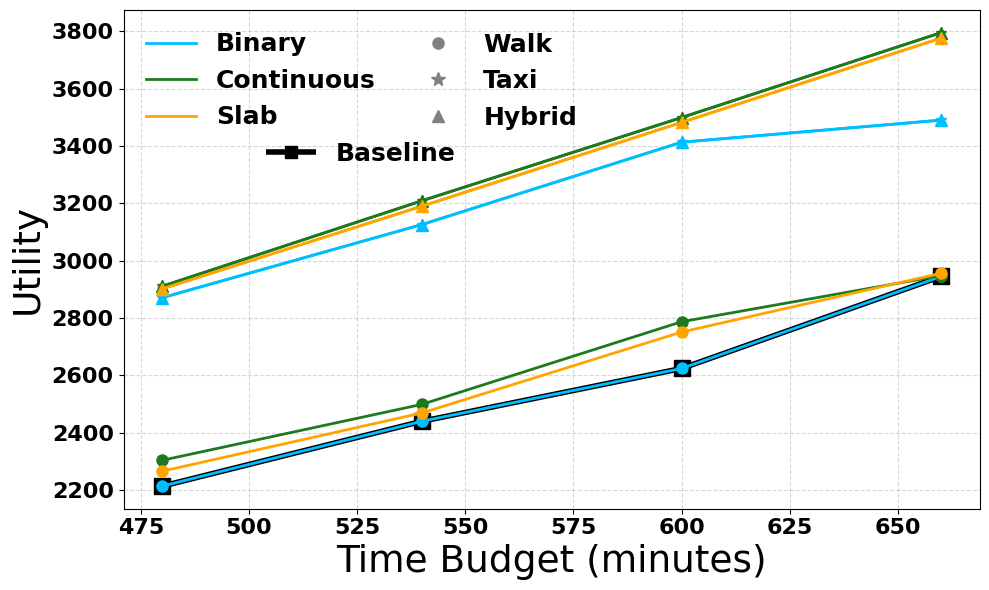
\includegraphics[width=\columnwidth]{plots/baseline_singleDay.png}
\caption{Comparison of \trip variants with baseline}
\label{fig:baseline-single}
\end{figure}

\subsection{Comparison with Baseline}

We first experiment to see the performance of \trip against the baseline.
Figure~\ref{fig:baseline-single}\footnote{This and all subsequent graphs use a combination of line colors for utility variants and point shapes for transportation modes. Since there are 3 utility variants and 3 transportation modes, a combination of these legends produces the 9 \trip variants. For example, since Binary is represented by cyan-colored lines and Walking by circles, a cyan-colored line with circles represent the Binary Walking variant of \trip.}
shows the utility scores across different time budgets under a high cost budget scenario (100000 units) for the city of Osaka for a single day.
As expected, utility increases with increasing time budget, since there is more time to visit more POIs.
Notably, the \trip Binary-Walking variant closely replicates the behavior of the baseline model, validating its correctness and fairness for comparative purposes. The other models, especially the Hybrid mode ones, outperform the baseline significantly.
Since the cost budget is very high, the utility scores of Taxi match those of Hybrid.

%Overall, the plot effectively highlights how our approach—especially the allowance for partial POI visits and the use of flexible transport—leads to significantly improved itinerary recommendations, both in terms of utility and adaptability to real-world constraints.

\begin{figure}[t]
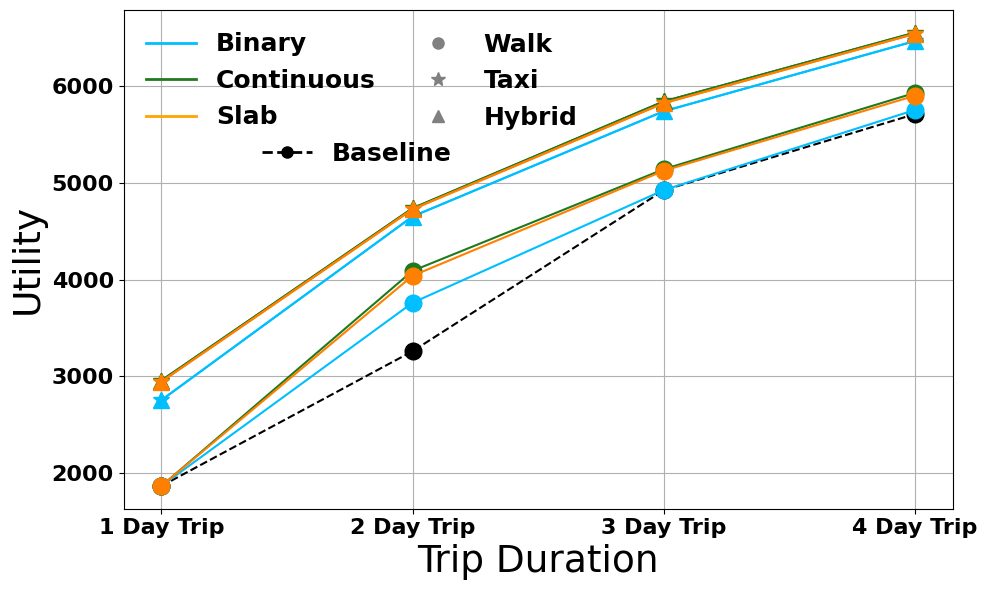
\includegraphics[width=\columnwidth]{plots/baseline_multiDay.png}
\caption{Comparison against baseline for multi-day trips}
\label{fig:baseline-multi}
\end{figure}

We next experiment with multi-day itinerary on Osaka for a very high cost budget of 100000 to ensure that cost is not a limiting factor for the baseline.
Each day was assigned a time budget of 8 hours.
Figure~\ref{fig:baseline-multi} shows the results for 1 to 4 days.
The baseline utilities were calculated by creating daily itineraries one after another, making sure not to repeat any POIs from previous days, and summing up the utilities.
The \trip variants run optimized multi-day planning models and, consequently, perform much better. Given the consistent and significant advantage of \trip over the baseline, we chose to leave the baseline out of future comparisons.

\begin{figure*}[t]
    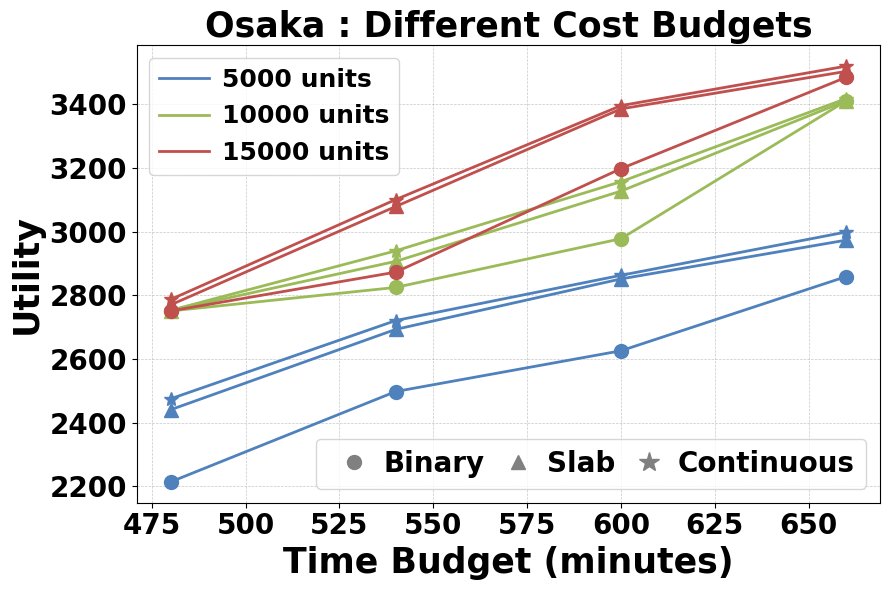
\includegraphics[width=0.33\textwidth]{plots/exp1-osaka.png}
    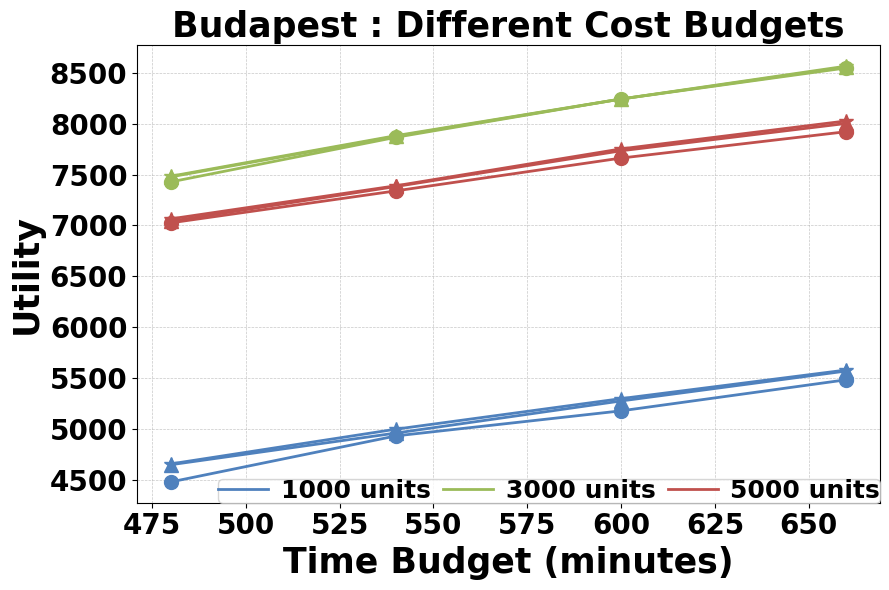
\includegraphics[width=0.33\textwidth]{plots/exp1-budapest.png}
    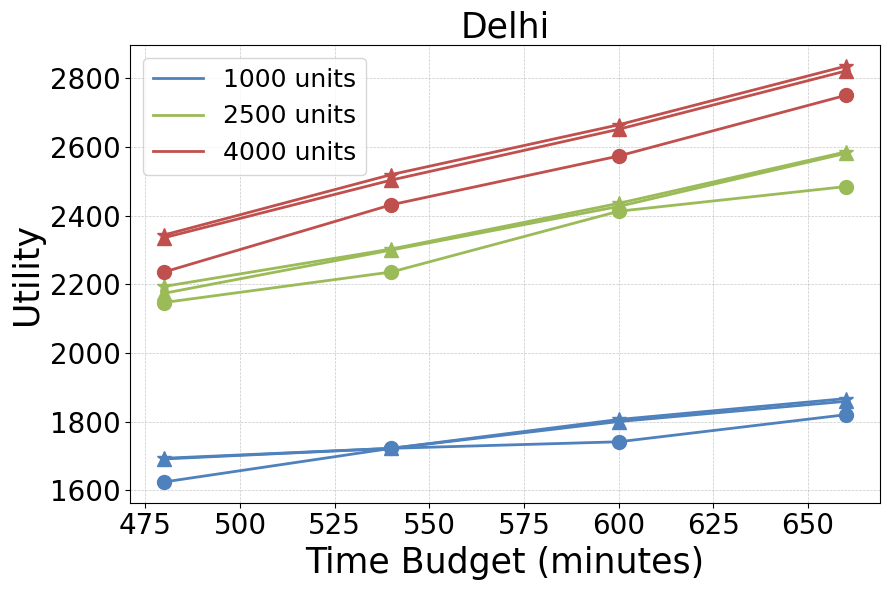
\includegraphics[width=0.33\textwidth]{plots/exp1-delhi.png}
    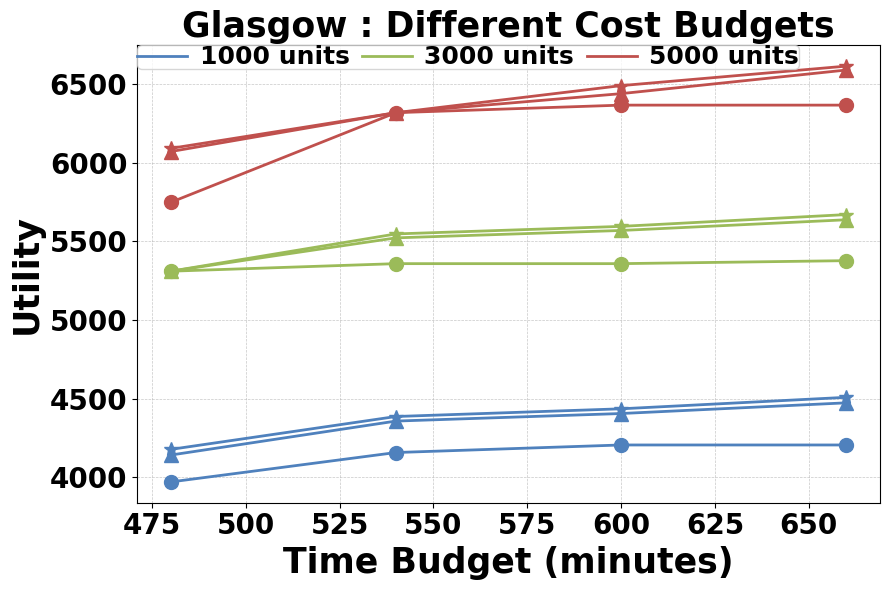
\includegraphics[width=0.33\textwidth]{plots/exp1-glasgow.png}
    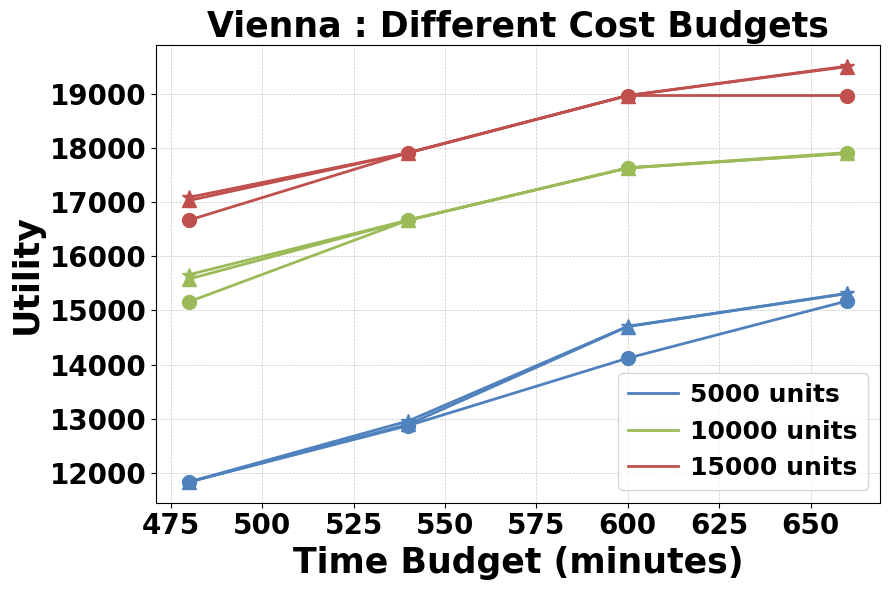
\includegraphics[width=0.33\textwidth]{plots/exp1-vienna.png}
    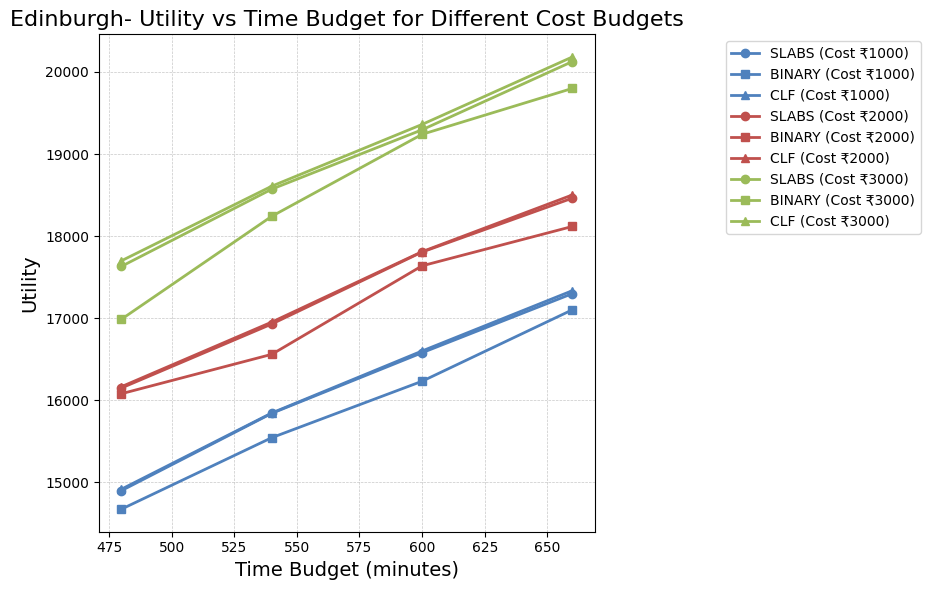
\includegraphics[width=0.33\textwidth]{plots/exp1-edinburgh.png}
    \caption{Utility variation with different time and cost budgets for 6 cities}
    \label{fig:cities}
\end{figure*}

\subsection{Multiple Cities}

Figure~\ref{fig:cities} shows the results of single day tour planning for 6 different cities under various time and cost budgets for different utility variants for the Hybrid mode.
The time budget is varied within a practical range of 480 to 600 minutes, and the cost budget is chosen to be appropriately aligned with the economic characteristics of the city.
As expected, higher cost and time budgets allow for higher utilities.
The Continuous utility variant shows the best performance.
\ab{can we have utilization numbers here?}
Since the trends remain the same across the cities, we choose Osaka as a representative, and show all subsequent results for it only.

%This offers a broad perspective on how the system adapts to varying resource constraints in diverse urban environments. For the remainder of the analysis, we focus on the city of Osaka as a representative case with a time budget of 480 minutes and cost budget of 6000 units. Unless stated otherwise, the default time budget is varied within a practical range of 480 to 600 minutes, and the cost budget is chosen to be appropriately aligned with the economic characteristics of the city. This approach allows us to maintain clarity while drawing generalizable conclusions from representative trends observed in one city.

\subsection{Effect of Multi-modality}

\begin{figure}[t]
\centering
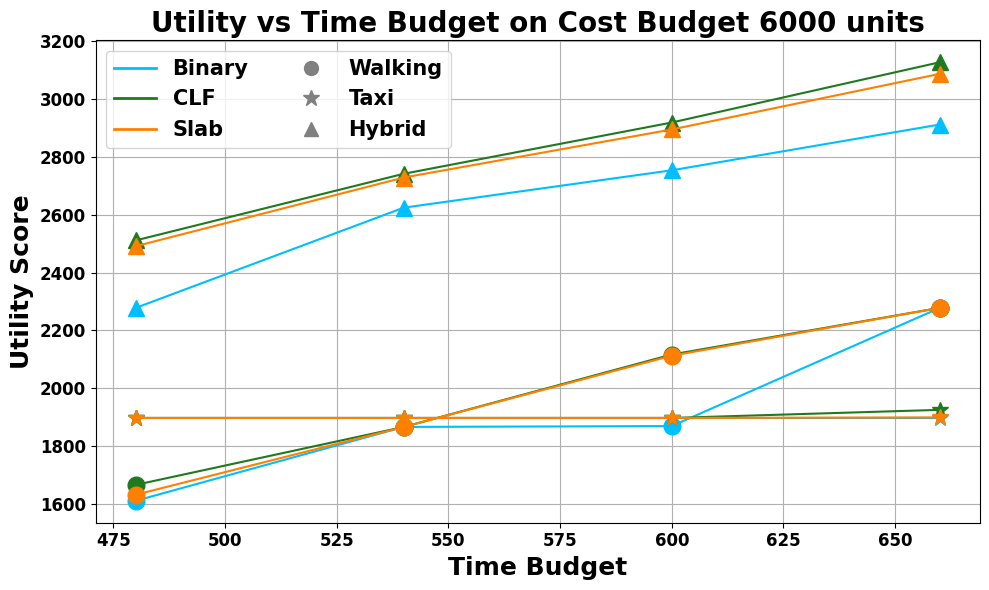
\includegraphics[width=\columnwidth]{plots/multimodality1.png}
(a) Fixed cost budget of 6000 units 
%\label{fig:mm1}
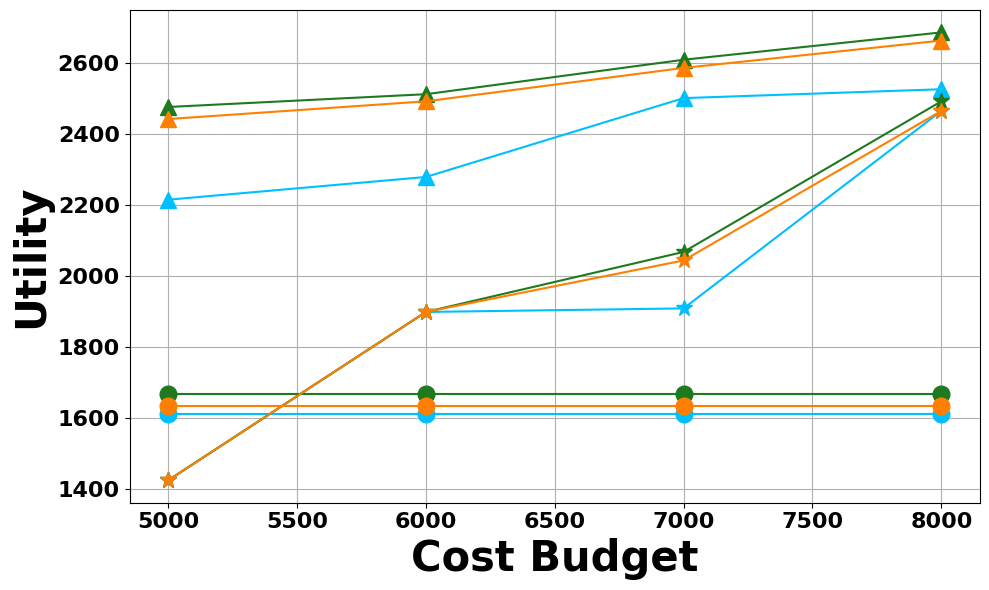
\includegraphics[width=\columnwidth]{plots/multimodality2.png}
(b) Fixed time budget of 480 minutes
\caption{Effect of transportation modes}
\label{fig:multi-modal}
\end{figure}

We next evaluate the effect of multiple modes of transport (Figure~\ref{fig:multi-modal}).
For a fixed cost budget (of 6000 units), the top graph shows that Hybrid is generally the best mode by a significant margin. This is intuitive since Hybrid chooses the best of both the worlds.
The utility obtained using only Taxi saturates after a while, since once the fixed cost budget is exhausted, it cannot visit any more POI.
The bottom graph shows the effect of increasing cost budget for a fixed time budget of 480 minutes.
Again, while Hybrid is the best mode, with larger cost budgets, the Taxi variant catches up quickly.
This is intuitive since a large cost budget allows the traveler to quickly visit multiple POIs by spending more on taxi.
Since walking does not incur any cost, for a fixed time budget, there is no effect of the cost budget on it, and the utility remains the same.
Among the utility variants, Continuous shows the best performance.

\ignore{

Figure~\ref{fig:multi-modal} distinguishes utility computation variants using different line colors. The travel modes are represented by markers: circle for Walking, star for Taxi, and triangle for Hybrid mode. For instance, a blue star denotes $TRIP\_T\_B$ mode, orange triangle denotes $TRIP\_H\_S$ mode and so on.
\ab{what is new in this graph in addition to Fig 5?}

This experiment was done to illustrate the impact of varying time and cost budgets on the utility achieved by different transportation modes in our itinerary planning framework. The top graph explores how increasing the time budget (with a fixed cost budget of 6000 units) affects utility. Here, we observe that the utility continues to increase for walking and hybrid modes, while it saturates for the taxi-only variant. This is because the taxi mode relies heavily on cost availability—once the fixed cost budget is consumed, additional time offers very little, to no further improvement. In contrast, the hybrid mode, which leverages both walking and taxi flexibly, consistently outperforms the single-mode options across all three TRIP variants, highlighting the effectiveness of our multi-modality feature.

The lower graph, which holds the time budget constant at 480 minutes while increasing the cost budget, further supports this observation: hybrid models adapt more efficiently to increased resource availability, maximizing utility better than single-mode approaches. In this case, the utility for walking-only variants remains saturated across all TRIP variants, as the potential gains from walking are constrained by the fixed time rather than by cost. Furthermore, a consistent trend is observed wherein the CLF (Continuous Linear Function) scoring model outperforms the slab-based model. Together, both graphs validate our design choices, demonstrating the combined advantages of multi-modal transportation and continuous utility modeling in enhancing itinerary quality.\\

}

%\noindent\textbf{Time Utilization}

\subsection{Time and Cost Profile}

\begin{figure}[t]
\centering
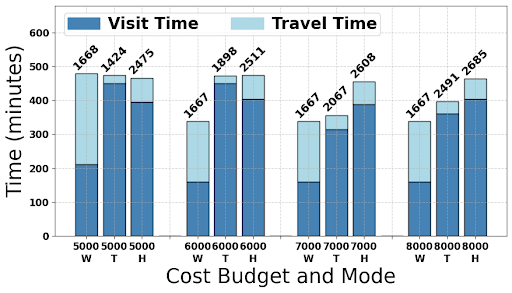
\includegraphics[width=\columnwidth]{plots/tu1.png}
(a) Fixed time budget of 480 minutes (Continuous)
%\caption{Travel Times vs Visit Times in 3 travel Modes on different cost budgets and fixed time budget (480 minutes)}
%\label{fig:TimeUtilization}
%\end{figure}
%\begin{figure}[th]
% 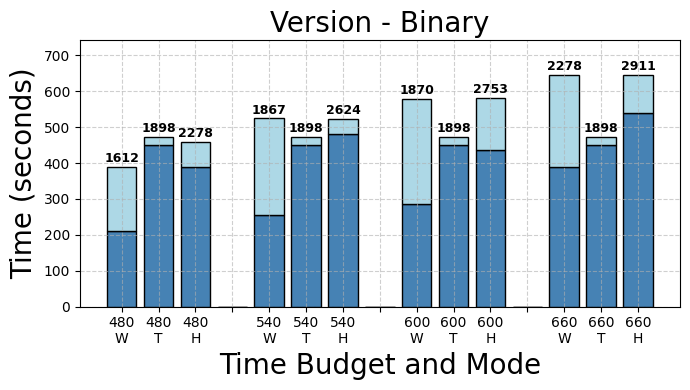
\includegraphics[width=0.23\textwidth]{plots/TIME_UTILIZATION_BINARY1.png}
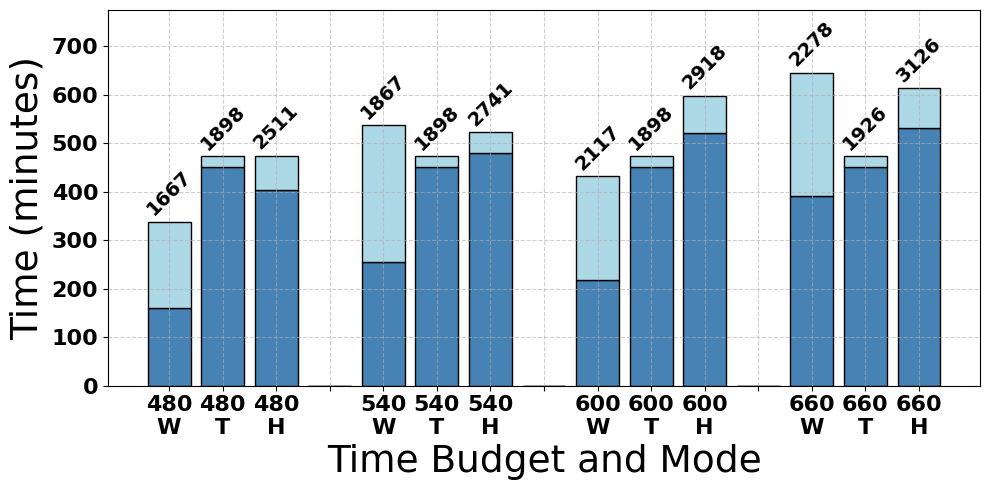
\includegraphics[width=\columnwidth]{plots/tu2.png}
(b) Fixed cost budget of 6000 units
% 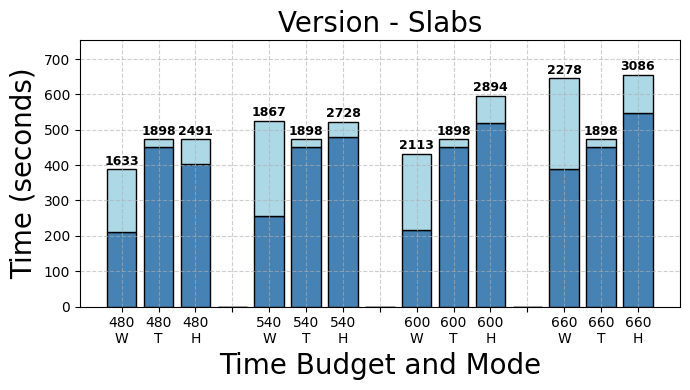
\includegraphics[width=0.23\textwidth]{plots/TIME_UTILIZATION_SLABS1.png}
% \centering
% 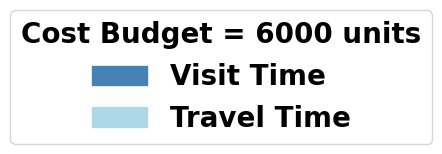
\includegraphics[width=0.25\textwidth]{plots/tu_legend2.png}
\caption{Time utilization (numbers on bars show utility scores)}
\label{fig:time-utilization}
\end{figure}

To understand the effects of different modes of transport even better, we next plot the time and cost utilization profiles.

Figure~\ref{fig:time-utilization} shows how the time is spent across visiting POIs versus traveling between POIs for different time and cost budgets.
Walking shows a high travel-to-visit time ratio, which is expected due to the slow nature of walking. A significant amount of time is, thus, spent in traveling. On the other extreme, Taxi minimizes travel time. Hybrid offers a solution which is mid-way, and achieves a more moderate ratio and a better utility.
Across all variants, increasing time budget allowed better utilization of available time, with Hybrid mode consistently providing the most balanced performance. This highlights that optimizing for utility involves not just maximizing visit duration but also strategically balancing travel efficiency with multi-modal flexibility.

\ignore{

Figures~\ref{fig:TimeUtilization} and ~\ref{fig:TimeUtilization1} present a comparison of travel time versus visit time across the three TRIP variants---walking-only (TRIP\_W), taxi-only (TRIP\_T), and hybrid (TRIP\_H)---at a fixed time budget of 480 minutes and varying cost budgets and at a fixed cost budget of 6000 units and varying time budgets respectively. Across all three utility scoring versions, a clear trend emerges: TRIP\_W exhibits a high travel-to-visit time ratio, reflecting the slower nature of walking as a mode of transport. In contrast, TRIP\_T minimizes travel time due to exclusive reliance on taxis, thereby maximizing time spent at points of interest (POIs). The hybrid model, TRIP\_H, maintains a balanced ratio between travel and visit time, offering a compromise between the two extremes. While the taxi-only model may seem efficient in terms of maximizing visit time, earlier experiments have demonstrated that it is the hybrid TRIP\_H that achieves the highest overall utility. Across all variants, increasing time budget allowed better utilization of available time, with Hybrid mode consistently providing the most balanced performance across travel and visit times. This highlights that optimizing for utility involves not just maximizing visit duration but also strategically balancing travel efficiency with multi-modal flexibility. 

}

Further, the Hybrid mode consistently achieves high time utilization, utilizing more than 95\% of the time budget, across all time and cost budgets. 
The Taxi mode shows better time utilization with smaller time budgets. For a higher time budget, since the cost budget is fixed, it quickly exhausts the cost and, consequently, fails to utilize the rest of the available time.
With increasing cost budget, however, it again improves the time utilization.

\ignore{

Walking mode shows similar time utilization across all cost budgets, indicating its inability to enhance utility on increasing cost budgets whereas on increasing time budget, its time utilization gets improved. Taxi mode starts strong with \textbf{98.7\%} utilization at 480 minutes, but gradually declines to around \textbf{74--82\%} at higher time budgets, as surplus time isn’t fully utilized because taxi is a cost based mode of transportation and hence on constant cost budget, increasing time budgets result in decline of time utilisation. This trend is evident in the plot, where hybrid mode bars nearly touch the top, reflecting optimal usage, while walking and taxi modes leave more unused time. Thus, hybrid mode offers the most consistent time utilization.
\\

}

%\noindent\textbf{Cost Utilization}

\begin{figure}[t]
\centering
% 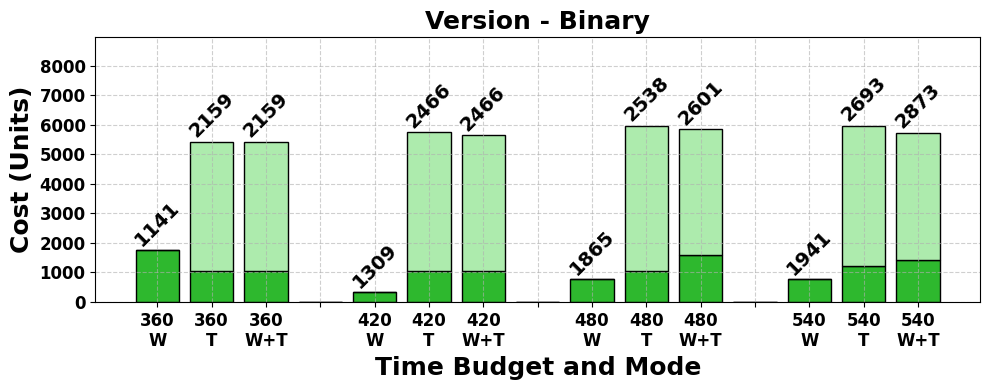
\includegraphics[width=\columnwidth]{plots/CU3_pkj.png}
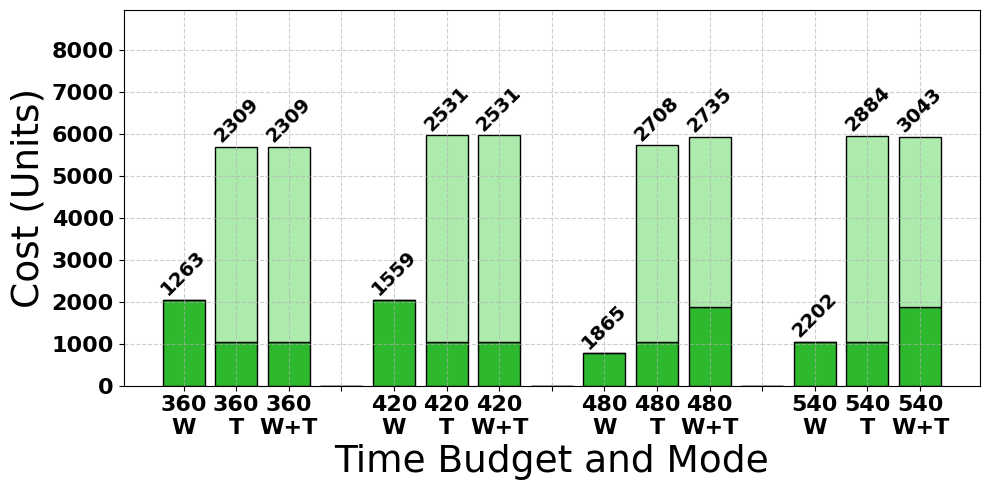
\includegraphics[width=\columnwidth]{plots/cu5.png}
(a) Fixed time budget of 480 minutes
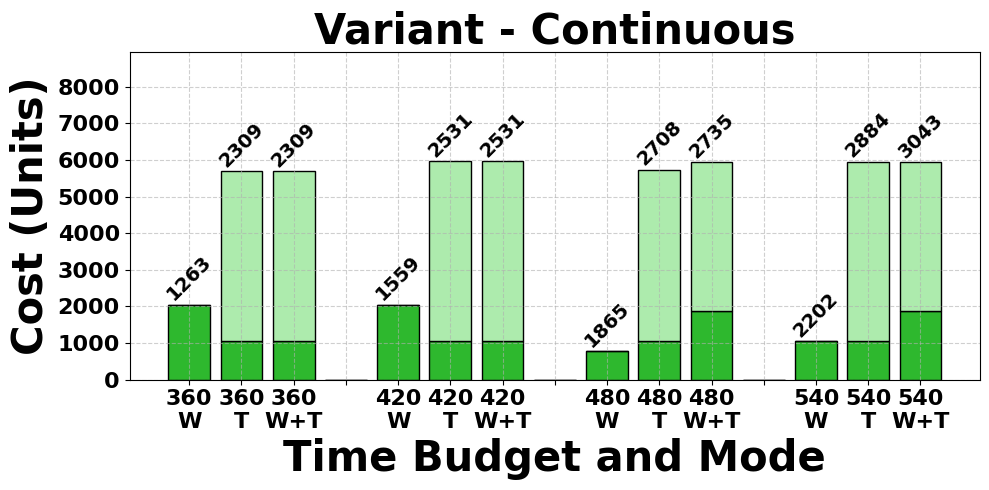
\includegraphics[width=\columnwidth]{plots/CU1.png}
(b) Fixed cost budget of 6000 units (Continuous)
% 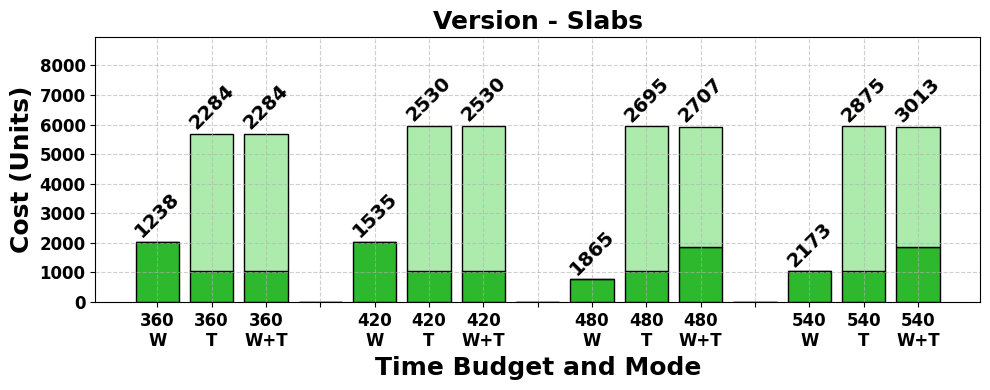
\includegraphics[width=\columnwidth]{plots/CU2_pkj.png}
%\caption{Travel Cost vs Visit Cost  in 3 travel Modes on different time budgets and fixed cost budget (6000 units)}
%\label{fig:CostUtilization1}
%\end{figure}
%\begin{figure}[th]
% 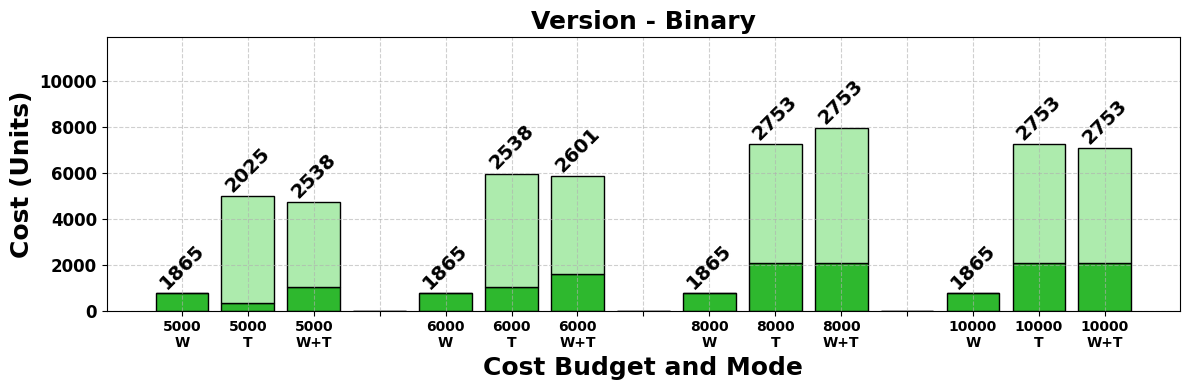
\includegraphics[width=\columnwidth]{plots/CU4_pkj.png}
% 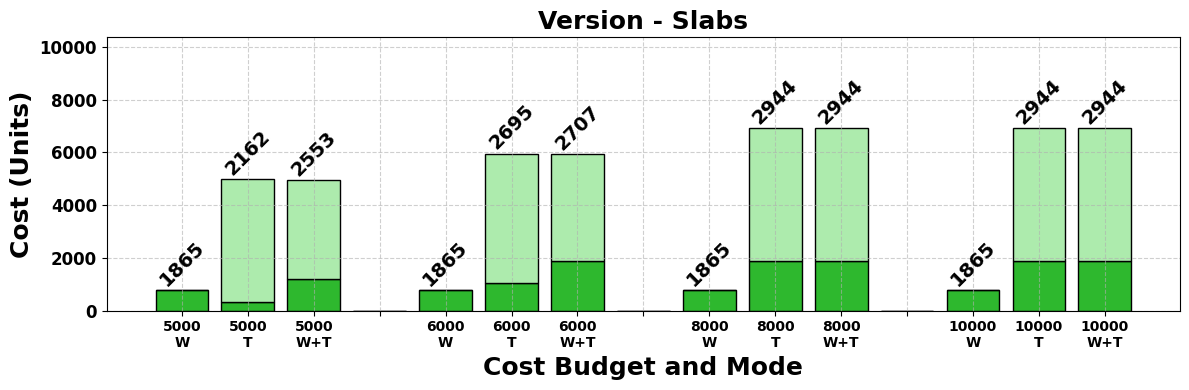
\includegraphics[width=\columnwidth]{plots/CU6_pkj.png}
% \centering
% 
\includegraphics[width=0.3\textwidth]{plots/cu5_legend.png}
\caption{Cost utilization (numbers on bars show utility scores)}
\label{fig:cost-utilization}
\end{figure}

Figure~\ref{fig:cost-utilization} shows the corresponding cost utilization profiles for the same experiments.
The POI visit costs are typically lower than the travel costs.
Hybrid offers a better ratio since it can visit more POIs.
Cost utilization, however, is not always an indicator of utility maximization.
The cost of visiting a POI is not always proportional to its utility.
In Taxi mode, although faster travel allows reaching distant POIs, the high travel cost often exhausts the budget before accessing faraway high-utility POIs.

\ignore{

\noindent These plots in Figures~\ref{fig:CostUtilization1} and ~\ref{fig:CostUtilization2} highlight that in itinerary optimization, cost utilization and utility maximization do not always go hand in hand — the system’s goal is to maximize utility under given constraints rather than simply minimizing or maximizing cost. The entrance (visiting) cost is not directly proportional to the utility score, as some high-utility POIs may have lower entrance costs while others with higher cost POIs may not contribute proportionally to utility. In pure taxi mode, although faster travel allows reaching distant POIs, the high travel cost often exhausts the budget before accessing faraway high-utility POIs, leaving unutilized time. In contrast, the hybrid mode (walking + taxi) leverages walking to access distant, high-utility POIs without incurring excessive travel costs, leading to higher utility even when total cost utilization appears lower.

The Cost utilization varies across travel modes and budget settings. With a fixed cost budget of 6000 units, walking mode exhibits cost utilization around \textbf{30\%} whereas Taxi and Hybrid  modes leads to higher cost utilizations of greater than \textbf{{95\%}}, showing improved resource usage due to multimodal flexibility. With a fixed time budget of 480 minutes, cost utilization in Hybrid mode increases with budget. Evidently, the cost utilisation of walking mode saturates across all cost budgets because no cost is incurred in this travel mode for transportation and all cost is utilized in entrance fee which is relatively less, while taxi mode shows similar trend as hybrid mode because it is a costly mode of transport and it utilizes the cost budget effectively.\\

}

%\noindent\textbf{Utility vs Time budget on different cost budgets}\\

\ignore{

\noindent \textbf{How to Read the Graphs}

\noindent In figure~\ref{fig:cities}, the graph uses \textbf{colored lines} to represent different \textbf{cost budgets}—for example in Osaka we use blue for 5000 units, green for 10000 units, and red for 15000 units—while \textbf{symbols on the lines} denote different versions of the itinerary planner: circle for \textit{Binary}, triangle for \textit{Slab}, and star for \textit{Continuous Function (CF)}. Each line formed by a specific combination of color and symbol indicates the \textbf{utility trend} for a particular planner variant at a given cost budget. For instance, in Osaka the \textbf{blue line with square markers} represents the performance of the \textit{Binary version} at a \textbf{cost budget of 5000 units}. This combination-based encoding enables a comparative analysis of planner performance across various time and cost constraints.\\

}

\ignore{

\noindent\textbf{Insights}

\noindent Figure~\ref{fig:cities} illustrates how the achieved utility varies across different combinations of time and cost budgets for the six cities in our dataset. A few consistent trends emerge across all cities. First, for a fixed cost budget, increasing the available time consistently leads to higher utility, highlighting the value of longer exploration durations. Second, for a given time budget, allocating a higher cost budget also results in improved utility, indicating the benefit of greater financial flexibility.\\

}

% % \newpage
% \noindent\textbf{Variation of Utility in Multi-day Itineraries}
% \begin{figure}[th]
% 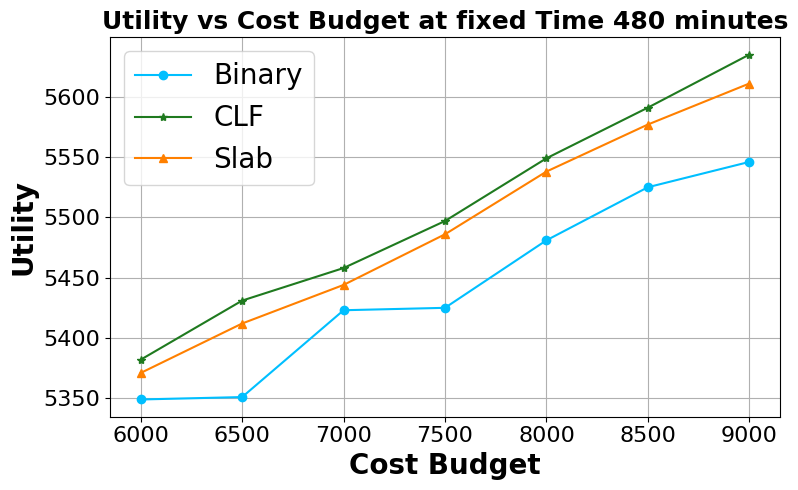
\includegraphics[width=0.45\textwidth]{plots/multiday1_pkj.png}
% % \end{figure}
% % \begin{figure}[th]
% 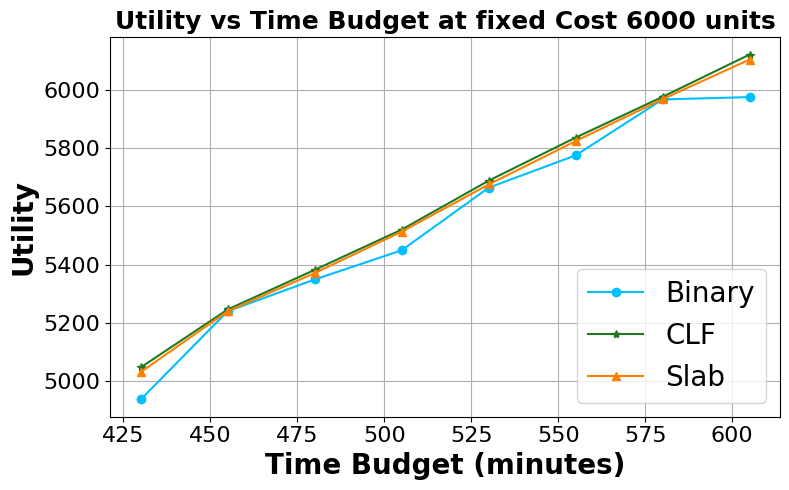
\includegraphics[width=0.45\textwidth]{plots/multiday2_pkj.png}
% \caption{Plots showing trends in Multi-day itineraries (3-day Trip) with Time Budget 480 minutes and Cost Budget 6000 units respectively}
% \label{fig:util_md}
% \end{figure}

% Figure ~\ref{fig:util_md} presents the utility trends for the multi-day variant of our itinerary planner for a 3 day trip. Similar to the single-day analysis, a consistent increasing trend in utility results is observed with fixed cost budget and increasing time budget and vice-versa, across the various formulations. Specifically, the utility achieved using the fractional variant is consistently higher than that of the binary variant, reaffirming the advantages of allowing partial visitations in enhancing overall experience. Furthermore, within the fractional formulations, the CLF (Continuous Linear Fractional) approach typically yields higher utility than the slab-based version, demonstrating its stronger capability to balance constraints and exploit budget flexibility effectively across multiple days of planning. However slabbed version works better than the binary version and thus it can be used to mathematically model the non linear utility functions in our problem which otherwise cannot be handled directly by ILP solvers and thus resulting in a better performance than the binary version.\\

\subsection{Multi-day Trips}

\begin{figure}[t]
\centering
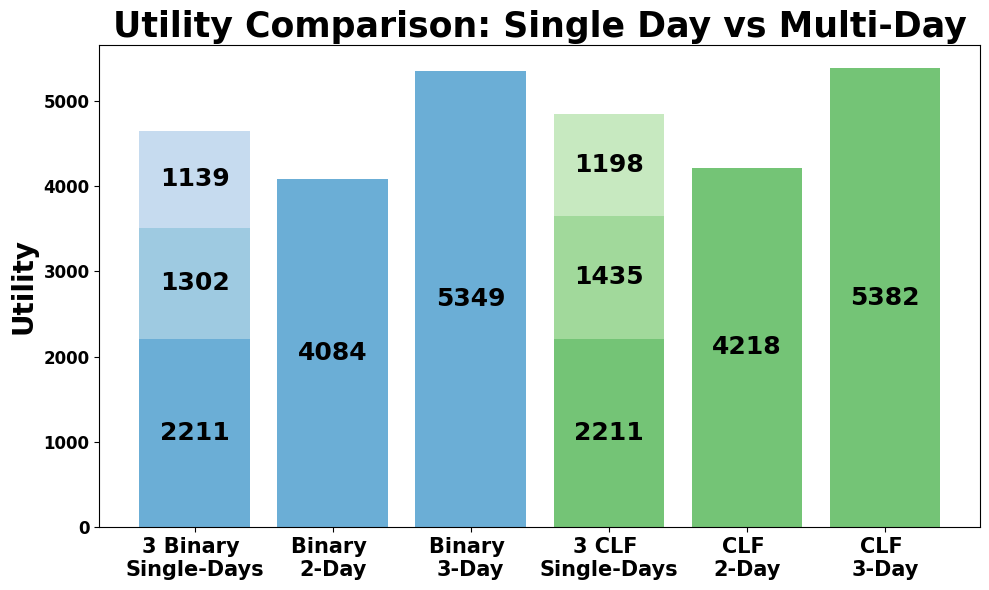
\includegraphics[width=0.45\textwidth]{plots/multivssingle.png}
\caption{Benefits of solving a single multi-day optimization problem against aggregating over several single-day itineraries}
\label{fig:multi-day}
\end{figure}

We next measure the effect of optimizing the utility for a multi-day itinerary against solving for single days, and summing the utilities.
Figure~\ref{fig:multi-day} shows the utility scores for the various settings for two utility variants (the Slab variant shows similar results as Continuous and is, hence, omitted).
The first bar shows the different utilities for each of the 3 days. The POIs visited in earlier days are set as must-avoid later.
The second bar solves a one-shot 2-day itinerary problem, while the third bar solves the same for a 3-day itinerary.
The time budget is set to 480 minutes per day.
The cost budget for a single day itinerary is 2000 units; thus, for a 2-day (respectively, 3-day) multi-day itinerary, it is set to 4000 (respectively, 6000 units).
As can be clearly shown, solving a single optimization problem for multiple days shows a much larger utility (10-15\% more) over solving for 3 separate days and aggregating the utilities.
Even for 2 days, the gain in utility is around 15\%.

\ignore{

Figure~\ref{fig:multi-day} illustrates a comparison of total utility achieved with different trip planning configurations: aggregated 3 single-day trips versus actual 2-day and 3-day multi-day itineraries, optimized for both Binary and CLF versions. In this experiment, each day was assigned an equal time budget of 480 minutes. For single-day trips, the cost budget was uniformly set at 2000 units per day, and for the multi-day cases, the aggregate cost budgets were similarly scaled: 4000 units for 2-day and 6000 units for 3-day trips. As a basis of comparison, the 3 single day trips were: source-to-hotel travel (bottom segment), hotel-to-destination travel (middle segment), and hotel-to-hotel travel (top segment). The last two segments are swapped for a fair comparison with 2-Day multiday trip version.\\

The results clearly demonstrate that multi-day planning consistently outperforms naive aggregation over single days. In the Binary variant, the 2-day multi-day plan has a score of 4084, whereas two single-day plans aggregated give lower cumulative utility. Similarly, in the 3-day variant, the multi-day plan has a score of 5349, much higher than the three single-day utilities summed up. The same is the case with the CLF variant, where the multi-day plans (4218 for 2-day, 5382 for 3-day) consistently beat the aggregated single-day utilities. This improved performance is due to the flexibility and optimization advantages of multi-day planning, where activities and itineraries can be optimized globally over multiple days as opposed to being restricted within independent daily plans. Thus, multi-day trip planning is not a single-day plan aggregation but a richer solution space that optimally exploits inter-day dependencies.\\

}

\subsection{Personalized Constraints}

\begin{figure}[t]
\centering
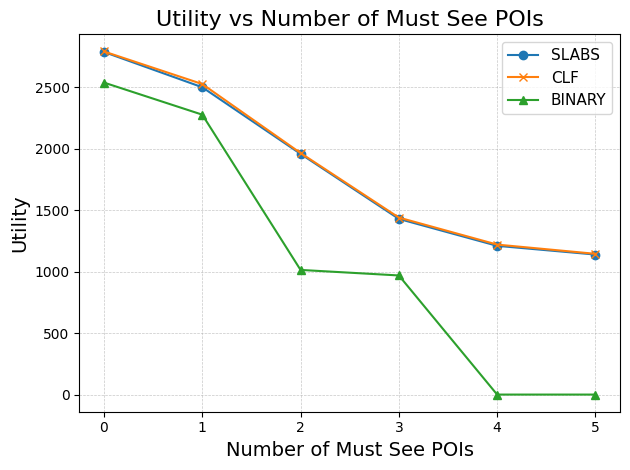
\includegraphics[width=0.24\textwidth]{plots/mustsee.png}
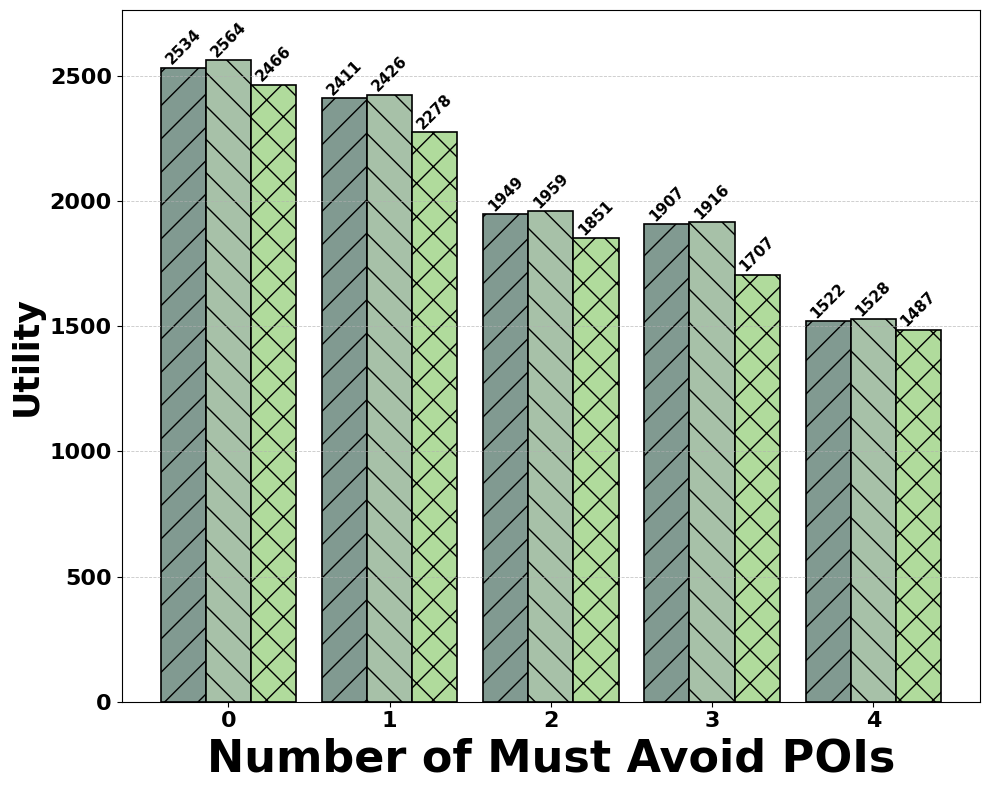
\includegraphics[width=0.24\textwidth]{plots/mustavoid.png}
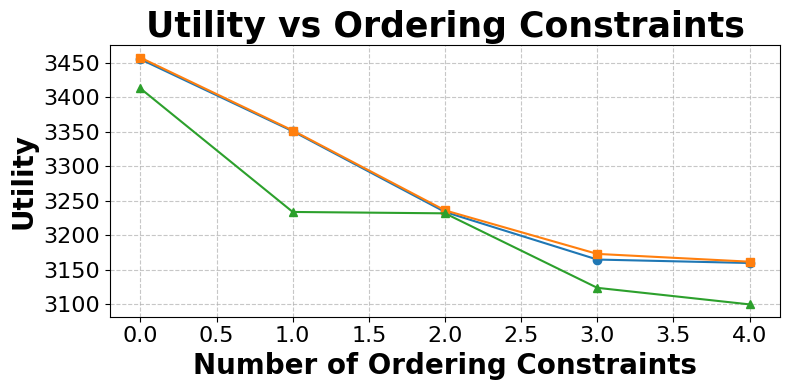
\includegraphics[width=0.24\textwidth]{plots/ordering.png}
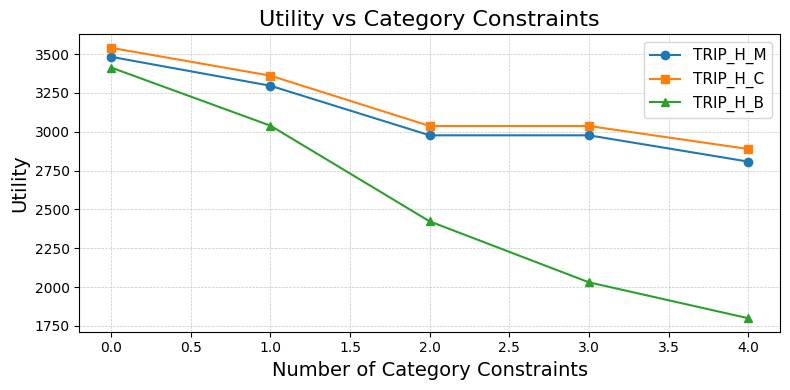
\includegraphics[width=0.24\textwidth]{plots/category.png}
% \raisebox{0.5\height}{
\includegraphics[width=0.24\textwidth]{plots/legend_personalized_pkj.png}}
\caption{Various personalized constraints}
\label{fig:personalizedconstraints}
\end{figure}

Figure~\ref{fig:personalizedconstraints} shows the results of various personalized constraints over the 3 utility variants.
In this study, a cost budget of 6000 units and a time budget of 480 minutes is fixed across all the cases.
With multiple must-see POIs fixed by the traveler, the utility falls, since there is not much scope for the solver to optimize. The same happens with multiple must-avoid POIs, although the decline is less sharp.
The same reduction in utility is observed with more number of ordering and category constraints.
Binary shows the sharpest drops since it has the least leeway; Slab and Continuous variants can partially visit a POI, and move to other POIs for better utility gain.

\ignore{

The impact of incorporating personalized constraints, that is, must-see, ordering, and category and must-avoid constraints, on overall utility is illustrated in the four graphs of figure ~\ref{fig:personalizedconstraints}. In this study a cost budget of 6000 units and a time budget of 480 minutes is fixed across all cases, it is evident that increasing the number of constraints leads to a decline in the achievable utility, as the solution space becomes more restricted. However, the extent of this reduction varies across the different formulations. Specifically, the CLF and slab variants show a relatively gradual decline in utility compared to the binary variant. This is primarily because the binary model lacks the flexibility to accommodate partial visits to POIs, thereby limiting its ability to adapt to tighter constraints. In contrast, the CLF and slab variants can better navigate these constraints by leveraging their ability to assign fractional visits, thus preserving higher utility under increasingly personalized user preferences.\\

}

%\noindent\textbf{Effect of Dynamic Re-planning}

\subsection{Dynamic Re-planning}

\begin{figure}[t]
    \centering
    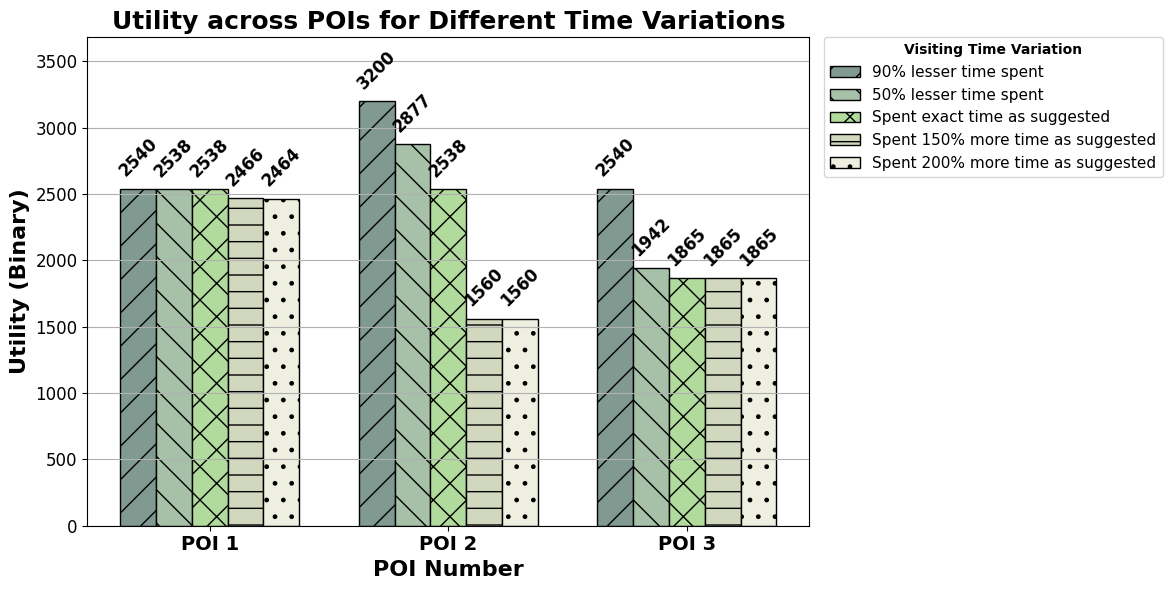
\includegraphics[width=0.50\textwidth]{plots/dynamic_pkj.png}
    \caption{Comparison of utility when tourist spends less or more time at a POI}
    \label{fig:dynamic}
\end{figure}

% \begin{figure*}[htbp]
%     \centering
%     % 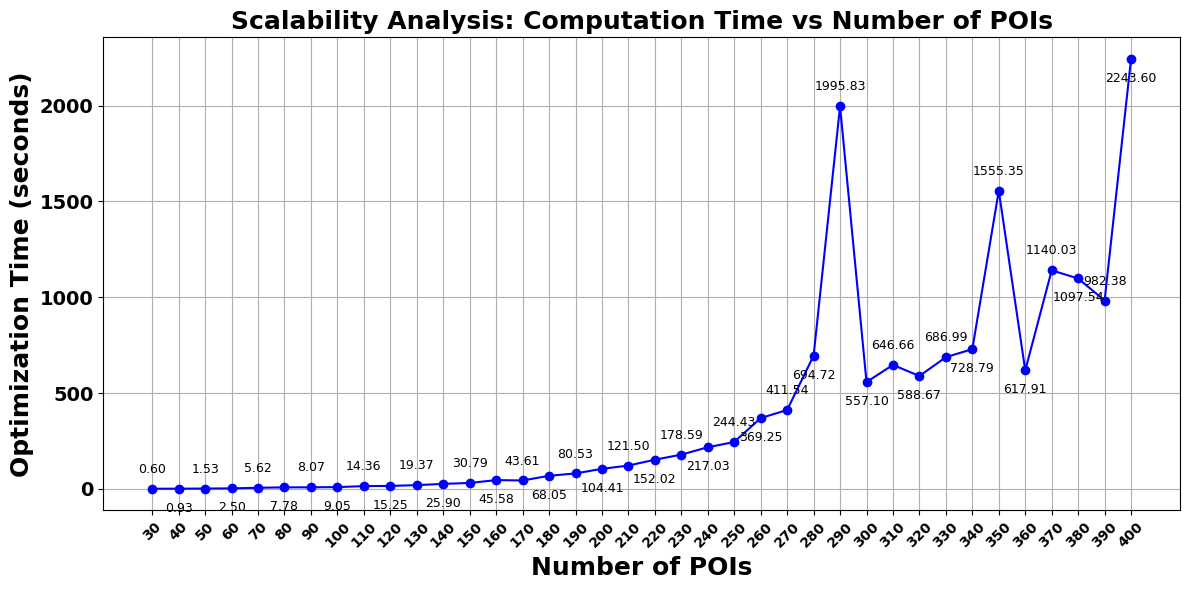
\includegraphics[width=\textwidth]{plots/scalability_pkj.png}
%     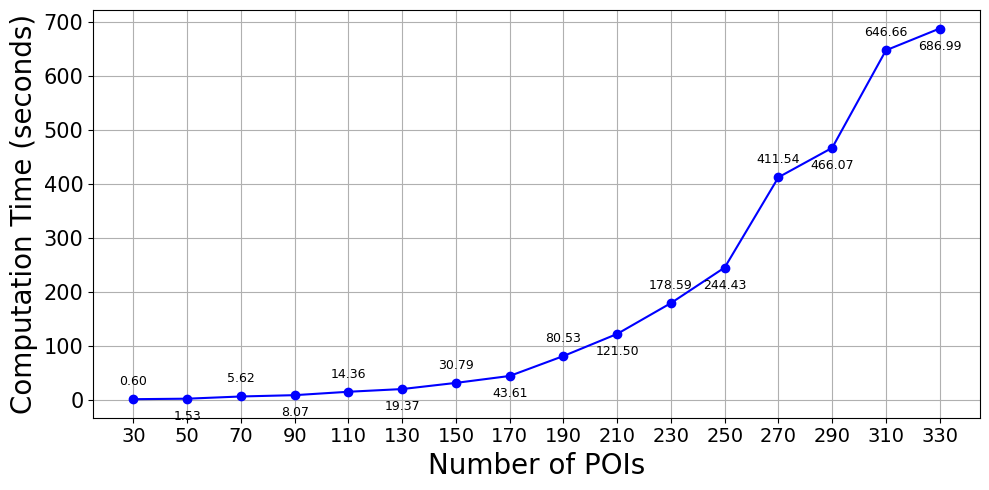
\includegraphics[width=\textwidth]{plots/scalability_new_pkj.png}
%     \caption{Time of computation on increasing number of POIs in single-day trips.}
%     \label{fig:scalability1}
% \end{figure*}

%\noindent\textbf{1. How to Read ~\ref{fig:dynamic_pkj}}

The next experiment captures the changes in utility when dynamic re-planning is done.
Figure~\ref{fig:dynamic} covers five different scenarios for a POI, according to the time spent in visiting it: (1)~\emph{50\% less}, i.e., when the traveler spends 50\% of the visit time prescribed, (2)~\emph{25\% less}, i.e., 75\% of the prescribed time, (3)~\emph{ontime}, i.e., when the traveler spends the exact prescribed time, (4)~\emph{50\% more}, i.e., 150\% of the prescribed time, and (5)~\emph{100\% more}, i.e., 200\% of the prescribed time.
The different groups specify the \emph{order} of the POI where the change is made (all other POIs spent the exact prescribed time).
The time and cost budget are 480 minutes and 6000 units respectively.
The optimal static itinerary consists of 4 POIs.
Our planner dynamically recalculates the itinerary by considering the actual time a user spends at each Point of Interest (POI) and the time taken to travel between them, in contrast to the initially suggested schedule.

The figure shows that the effect of spending a substantially different time on the first POI does not have much effect, since there is enough time for the planner to find another itinerary with a similar utility.
Similarly, spending less time in the third POI does not give a much better itinerary since there is not much scope to maneuver, given the time budget already spent. Spending a lot of extra time may, however, decrease the utility significantly, especially if this does not allow reaching the fourth and subsequent POIs.
The most amount of variability is visible for the second POI.
Spending lesser times results in re-planning significantly better itineraries, while spending much longer times results in lesser utility itineraries, despite re-planning.

Overall, this variation in utility values underscores the importance of adapting the itinerary based on real-time user behavior, demonstrating the effectiveness of our dynamically responsive planning approach.

\ignore{

%In all cases, travel times between any pair of POIs remain unaffected by user behaviour, and it takes the same time to travel by the user as suggested. Each POI has five bars, each representing different scenarios as stated above. Bar heights indicate utility levels, with values labeled on top. Distinct patterns and colors differentiate time-spent categories, as indicated in the legend.\\

%\noindent\textbf{2. Insights}

% \pri{Discuss about binary variant usage here}
Our planner dynamically recalculates the itinerary by considering the actual time a user spends at each Point of Interest (POI) and the time taken to travel between them, in contrast to the initially suggested schedule.  As shown in figure, at a time budget of 480 minutes and cost budget of 6000 units in TRIP\_H\_B variant, the \textbf{utility consistently decreases} as the time spent at a POI increases.

This trend can be explained as follows:

\begin{itemize}
    \item Spending \textbf{less time} at a POI allows the user to \textbf{save time}, which can be used to visit \textbf{additional POIs}, thereby increasing the overall utility.
    \item Conversely, as more time is spent at a single POI, the user has \textbf{less time available} to explore other POIs, resulting in a \textbf{decrease in total utility}.
\end{itemize}

\noindent This variation in utility values underscores the importance of adapting the itinerary based on real-time user behavior, demonstrating the effectiveness of our dynamically responsive planning approach.\\

}

%\noindent\textbf{Scalability}

\subsection{Scalability}

In this section, we test the scalability of our MILP solution in terms of running time for various parameters.

Figure~\ref{fig:number-of-pois} and Figure~\ref{fig:number-of-days} show that the time increases exponentially with number of POIs and number of days in the trip, which is expected for a linear programming solution.
Importantly, the computation times remain \emph{practical} even when the number of POIs or the number of days is very high.

\ignore{

To evaluate the scalability of our itinerary planning system, we examine how the computation time required to generate a complete itinerary varies with the number of Points of Interest (POIs) in a city, while keeping the time and cost budgets fixed at sufficiently accommodating values of 480 minutes and 6000 units respectively. As illustrated in Figure~\ref{fig:dynamic}, the observed increase in computation time with the number of POIs is expected, given that our approach is formulated as an Integer Linear Program (ILP). This growth aligns with the theoretical complexity of the underlying problem — a variant of the Team Orienteering Problem — which is known to be NP-Hard. Despite this, our formulation remains tractable for problem sizes typical of real-world tourist cities. Despite this theoretical complexity, our system demonstrates strong practical performance. For instance, with approximately 180 POIs, the itinerary is generated in under 1 minute. Even with nearly 260 POIs, the computation time remains approximately 5 minutes. These results highlight that, for realistically sized cities, our system maintains high computational efficiency, making it a viable and scalable solution for real-world deployment.
% \pri{was the content for optimal utility vs AI added?}

}

\begin{figure}[t]
    \centering
    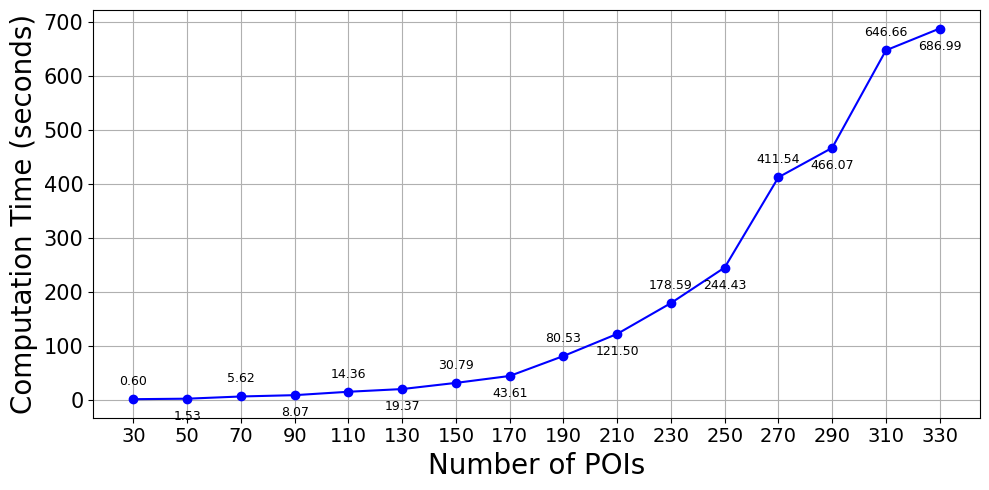
\includegraphics[width=\columnwidth]{plots/scalability_new_pkj.png}
    \caption{Scalability with number of POIs}
    \label{fig:number-of-pois}
\end{figure}

\ignore{

In order to further check the scalability of the suggested itinerary planning system, we designed an experiment by increasing the number of days in the trip as shown in figure~\ref{fig:scalability2}. The time budget was chosen as 480 minutes per day and the cost budget for day 1 was kept 2000 units for the whole trip. We kept increasing the cost budget by 2000 units on each subsequent day. The experiment was run for trips from 1 to 6 days.

The Time of Computation (TOC) for each case was measured. As anticipated, the TOC grows large as the days increase, mostly owing to the exponential increase in the solution space with the more days. It thereby aptly captures the scalability issue while the computation time still remains scalable for a practical constraint.\\
\nl{Please read this once}

}

\begin{figure}[th]
    \centering
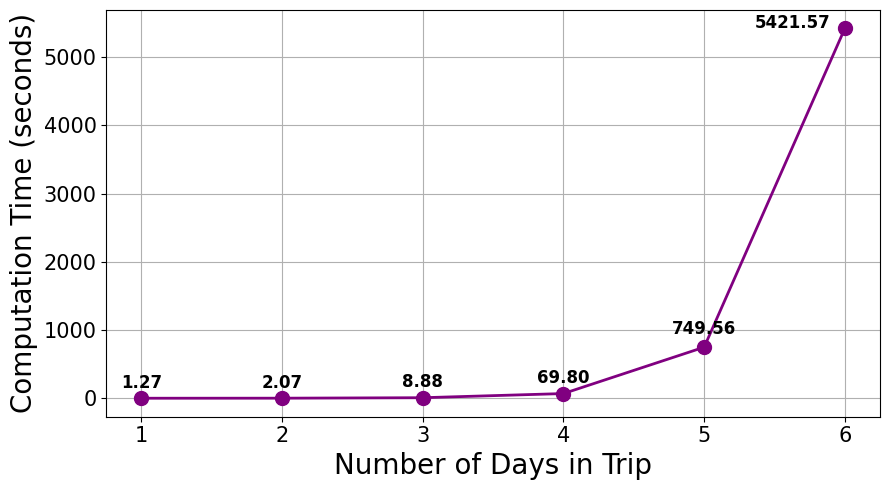
\includegraphics[width=0.4\textwidth]{plots/scalability_multiday.png}
     \caption{Scalability with number of days in multi-day trips}
    \label{fig:number-of-days}
\end{figure}

% \begin{figure*}[htbp]
%     \centering
%     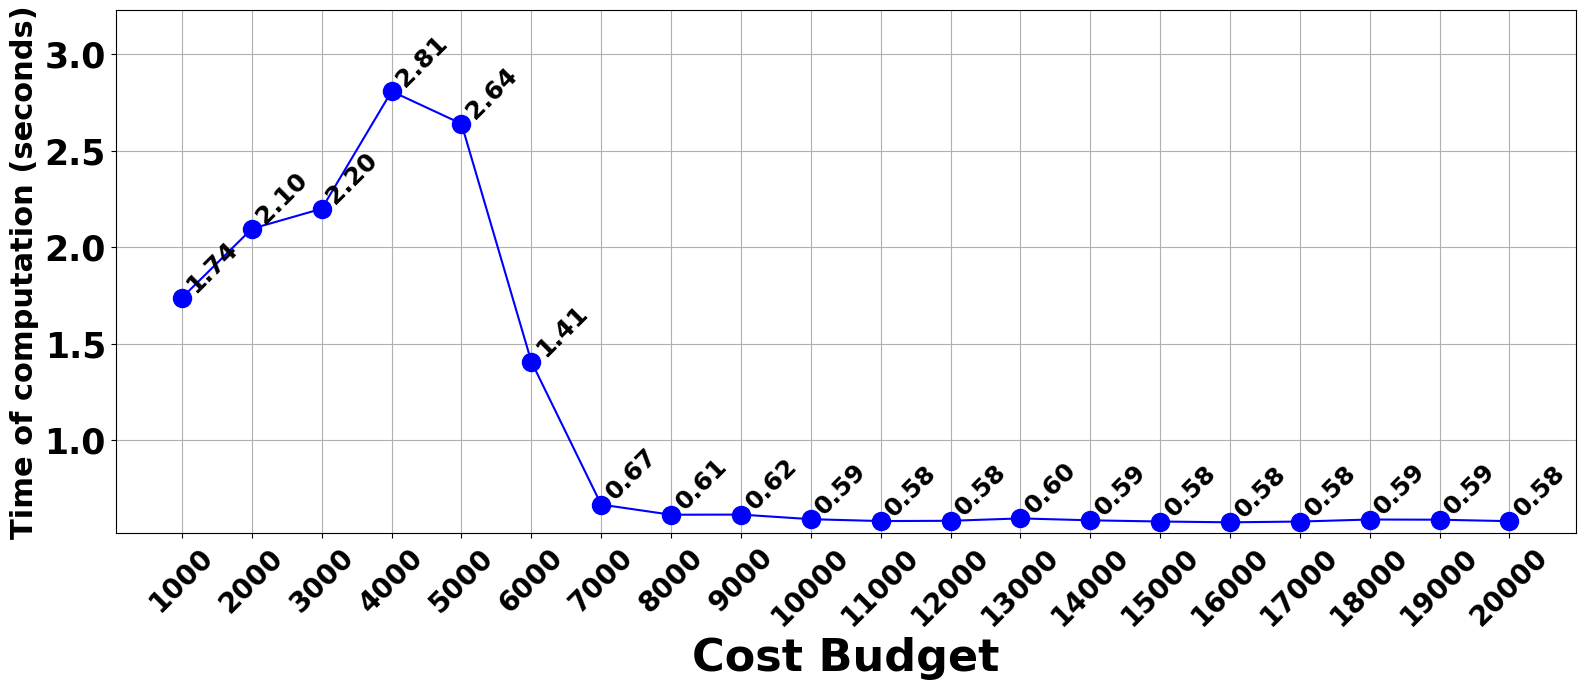
\includegraphics[width=\textwidth]{plots/costbudgetvstoc.png}
%     \caption{Time of computation on increasing cost budget at fixed time budget 480 minutes}
%     \label{fig:costbudgetvstoc}
% \end{figure*}



% \begin{figure*}[htbp]
%     \centering
%     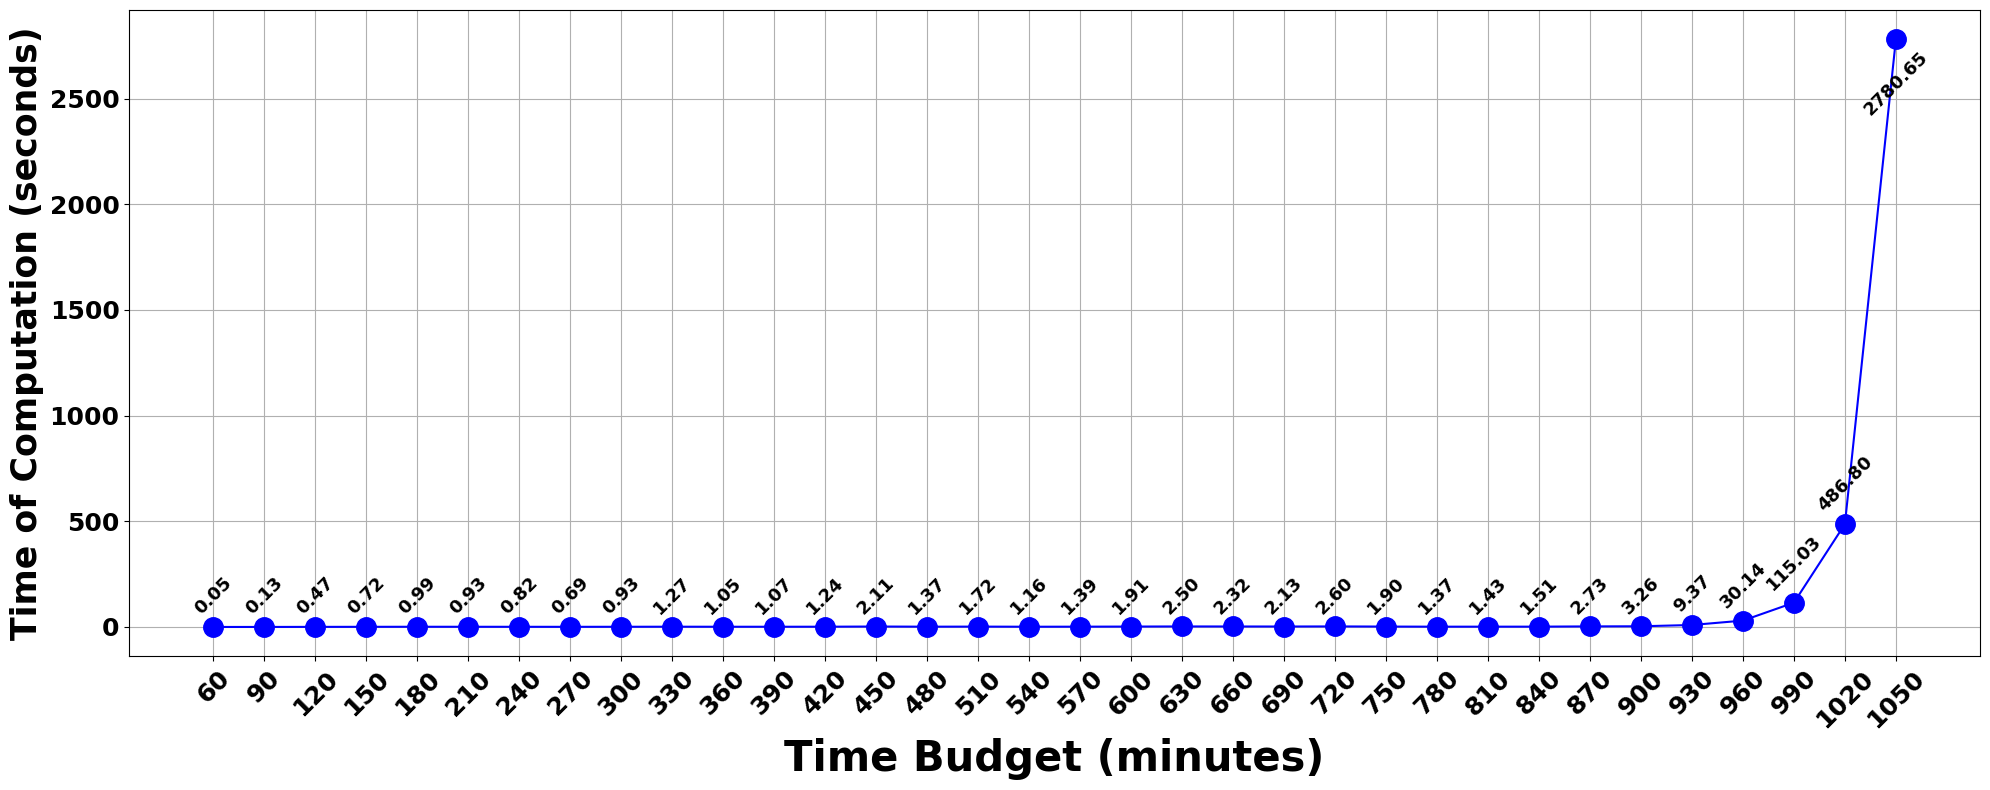
\includegraphics[width=\textwidth]{plots/timebudgetvstoc.png}
%     \caption{Time of computation on increasing time budget at fixed cost budget 6000 units}
%     \label{fig:timebudgetvstoc}
% \end{figure*}

We next show the change in computation time when the cost and time budget change.
As shown in Figure~\ref{fig:cost-budget}, for extremely low cost budgets, the time taken is small, but it increases rapidly with increasing cost budget. This is due to the fact that more choices become available when the cost budget increases. However, once the cost budget exceeds a threshold, the solver can effectively ignore about it, since almost all solutions become feasible in terms of cost.
Similarly, the computation time remains very low, unless the time budget is extremely high (Figure~\ref{fig:time-budget}) since only then almost all solutions become feasible in terms of time.

\ignore{

\noindent The computational efficiency of the suggested itinerary optimization model was tested against both cost budget and time budget changes. In figure~\ref{fig:costbudgetvstoc}, as the cost budget rises from low values, the computation time records a minimal increment and hits a plateau, perhaps as the solution space complexity is raised. But above some cost budget limit (approximately 6000), the computation time levels off and is always low for a broad range of cost budgets. This indicates that after the feasible space is large enough, further increases in the budget no longer have a major effect on solver performance. On the contrary, figure~\ref{fig:timebudgetvstoc} illustrates that computation time is much less robust to the time budget. While initially the increase in time budget leads to only a gradual rise in computation time, beyond 900 minutes, the solver time escalates sharply, indicating the rapidly growing complexity of exploring a significantly larger feasible space. Particularly towards the upper end, computation time skyrockets, pointing out that cost budget is less important than time budget in defining the computational complexity of the problem.

}

\begin{figure}[t]
    \centering
    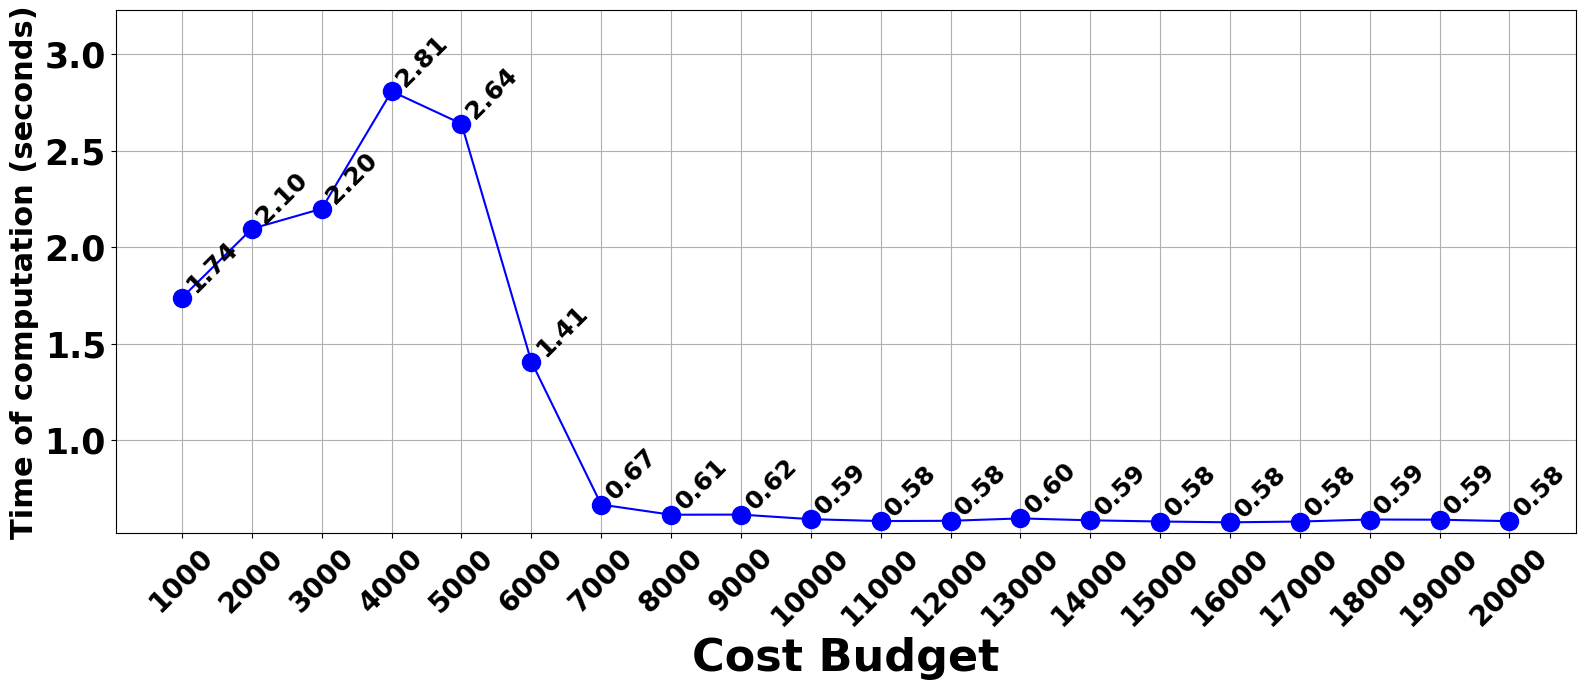
\includegraphics[width=\columnwidth]{plots/costbudgetvstoc.png}
    \caption{Time of computation on increasing cost budget at fixed time budget 480 minutes}
    \label{fig:cost-budget}
\end{figure}

\begin{figure}[t]
    \centering
    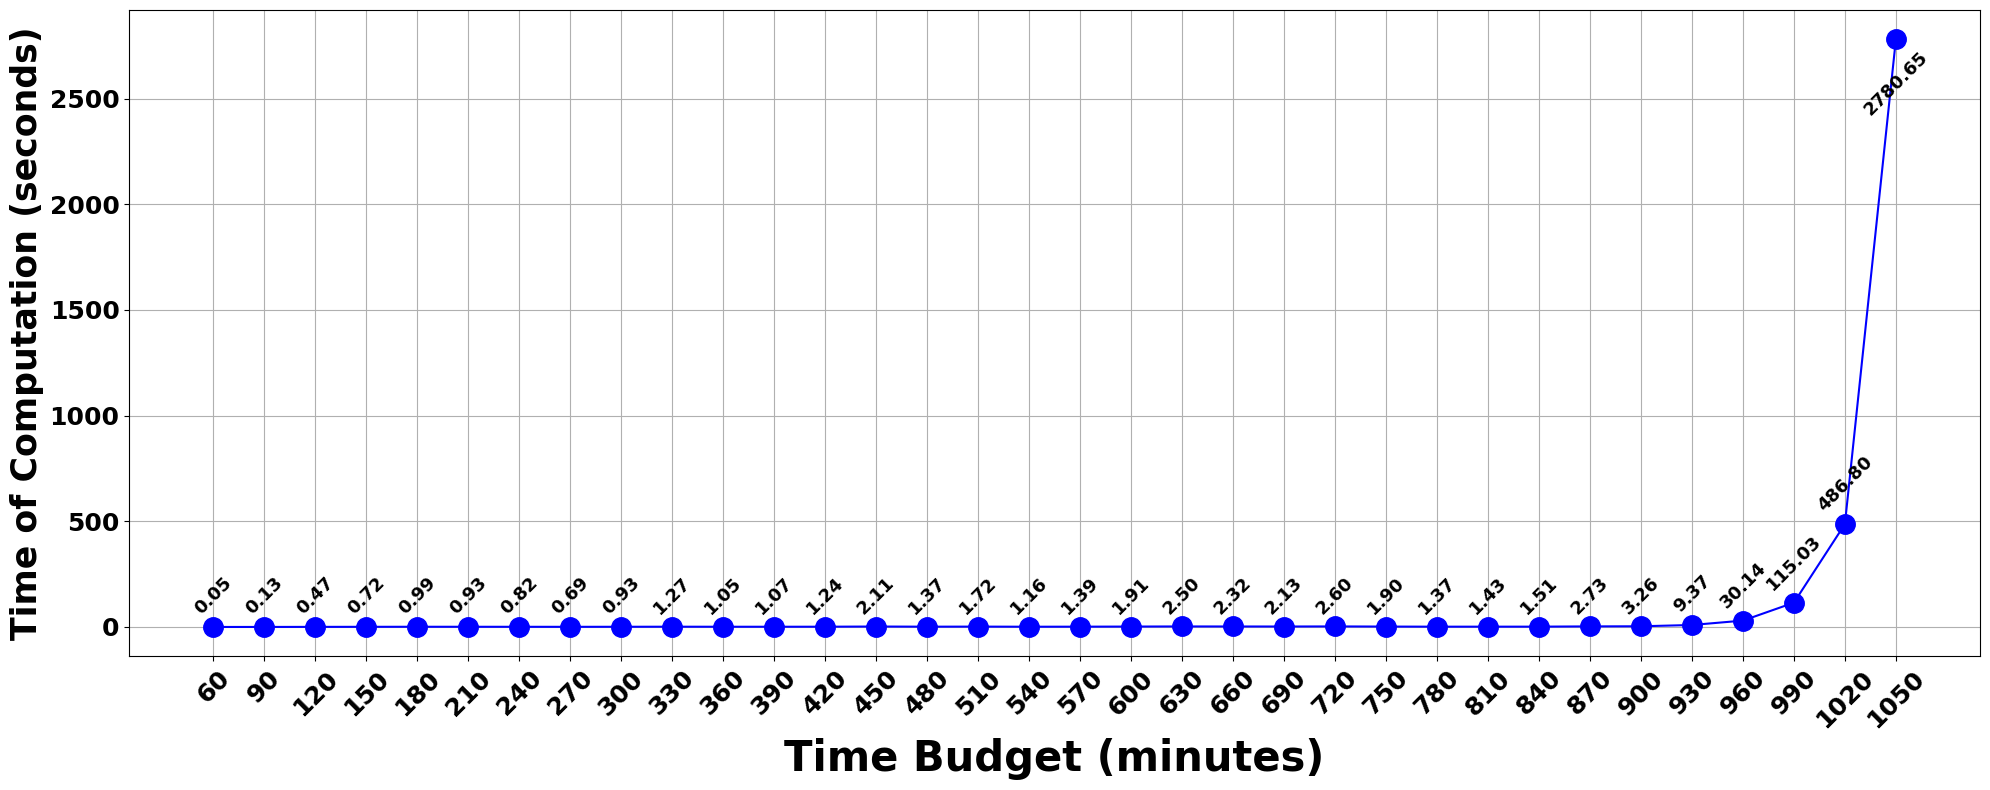
\includegraphics[width=\columnwidth]{plots/timebudgetvstoc.png}
    \caption{Time of computation on increasing time budget at fixed cost budget 6000 units}
    \label{fig:time-budget}
\end{figure}

%\noindent\textbf{Conclusions}\\

%\ab{Please read this section!}\\

%As shown in Figure~5, we are able to successfully replicate the existing baseline version (\texttt{TRIP\_W\_B}).

\subsection{Summary of Experimental Results}

Overall, our experimental results provide the following insights.
The \trip variants outperform the baseline significantly.
The Hybrid is the best mode of transport.
The Continuous utility variant gives slightly better results than the Slab variant, and both of them outperform the Binary variant due to lack of flexibility for the Binary variant.
Optimizing for multiple days in one shot gives significantly better results than solving for single days, and adding them up.
Personalized constraints are handled efficiently by our \trip solution.
Dynamic re-planning can increase the utility when there is scope to maneuver the rest of the plan.
Finally, \trip solver, despite being a MILP solution, is practical.

\ignore{

Moving forward, as observed in all the figures of this section, both the Continuous and Slab variants of the itinerary planner demonstrate superior performance over the Binary variant by enabling users to achieve higher utility values. This provides sufficient evidence to establish that the Continuous and Slab variants are more effective than the Binary variant. However, while the Continuous variant generally yields higher utility compared to the Slab variant, it is not appropriate to directly compare these two approaches. The Slab variant was specifically introduced to address the challenge of modeling non-linear utility functions, which cannot be directly handled by ILP solvers. By discretizing such non-linear functions into multiple slabs, they can be mathematically formulated and optimized within the ILP framework. Therefore, Continuous and Slab variants serve distinct purposes and address different problem complexities; any direct comparison in terms of utility alone would be misleading. Both variants offer unique advantages in handling different utility modeling scenarios, and hence, we continue the subsequent analysis with both, without declaring either one superior over the other.

}
